\startchapter{Experimental Setup}
\label{chapter:Exp}

The spatial interpolation methods will be evaluated on two datasets. The first is a synthetic dataset produced by a physics-based soil simulation modelling the movement and biodegradation of hydrocarbons in the soil.This dataset is used to evaluate the models across a variety of conditions, including measurement noise, sensor count, soil parameter noise, measurement frequency and measurement dropout. A subset of the simulated dataset is also used to tune the hyperparameters of the interpolation algorithms. The second dataset consists of real measurements from a contaminated site on the Canadian Prairies. Due to the limited number of available samples, these results serve primarily to validate findings from the simulated dataset. The real-world data is examined first to establish the format and context that motivates the design of the simulated dataset.

\section{Real-World Data}
\label{sec:real_data}

The real measurement dataset was collected from an active biostimulation remediation site on the Canadian Prairies. It consists of 27 data samples acquired from 11 measurement stake locations distributed across the contaminated area. Each stake hosts a sensor array at depths of 1.5~m, 2.5~m, and 3.5~m below the surface. These depths were chosen to capture the vertical extent of the PHC plume, which tends to migrate downward through the soil column under the influence of gravity and precipitation-driven leaching~\cite{PHC_movement_source}.

At each depth, a Beer-Lambert sensor measures absorbed light through the air to determine PHC concentration at 30-minute intervals~\cite{beerLambertSensor}. To reduce measurement noise while preserving the underlying remediation dynamics, these raw readings are aggregated into 12-hour averages, yielding two observations per depth per day at each stake location. Each data sample therefore consists of a time series of PHC concentration measurements at three depths from a single stake location, sampled at 12-hour increments, as shown in Fig. \ref{fig:realMeas_intro}.

 \begin{figure}[H]
 \centering
 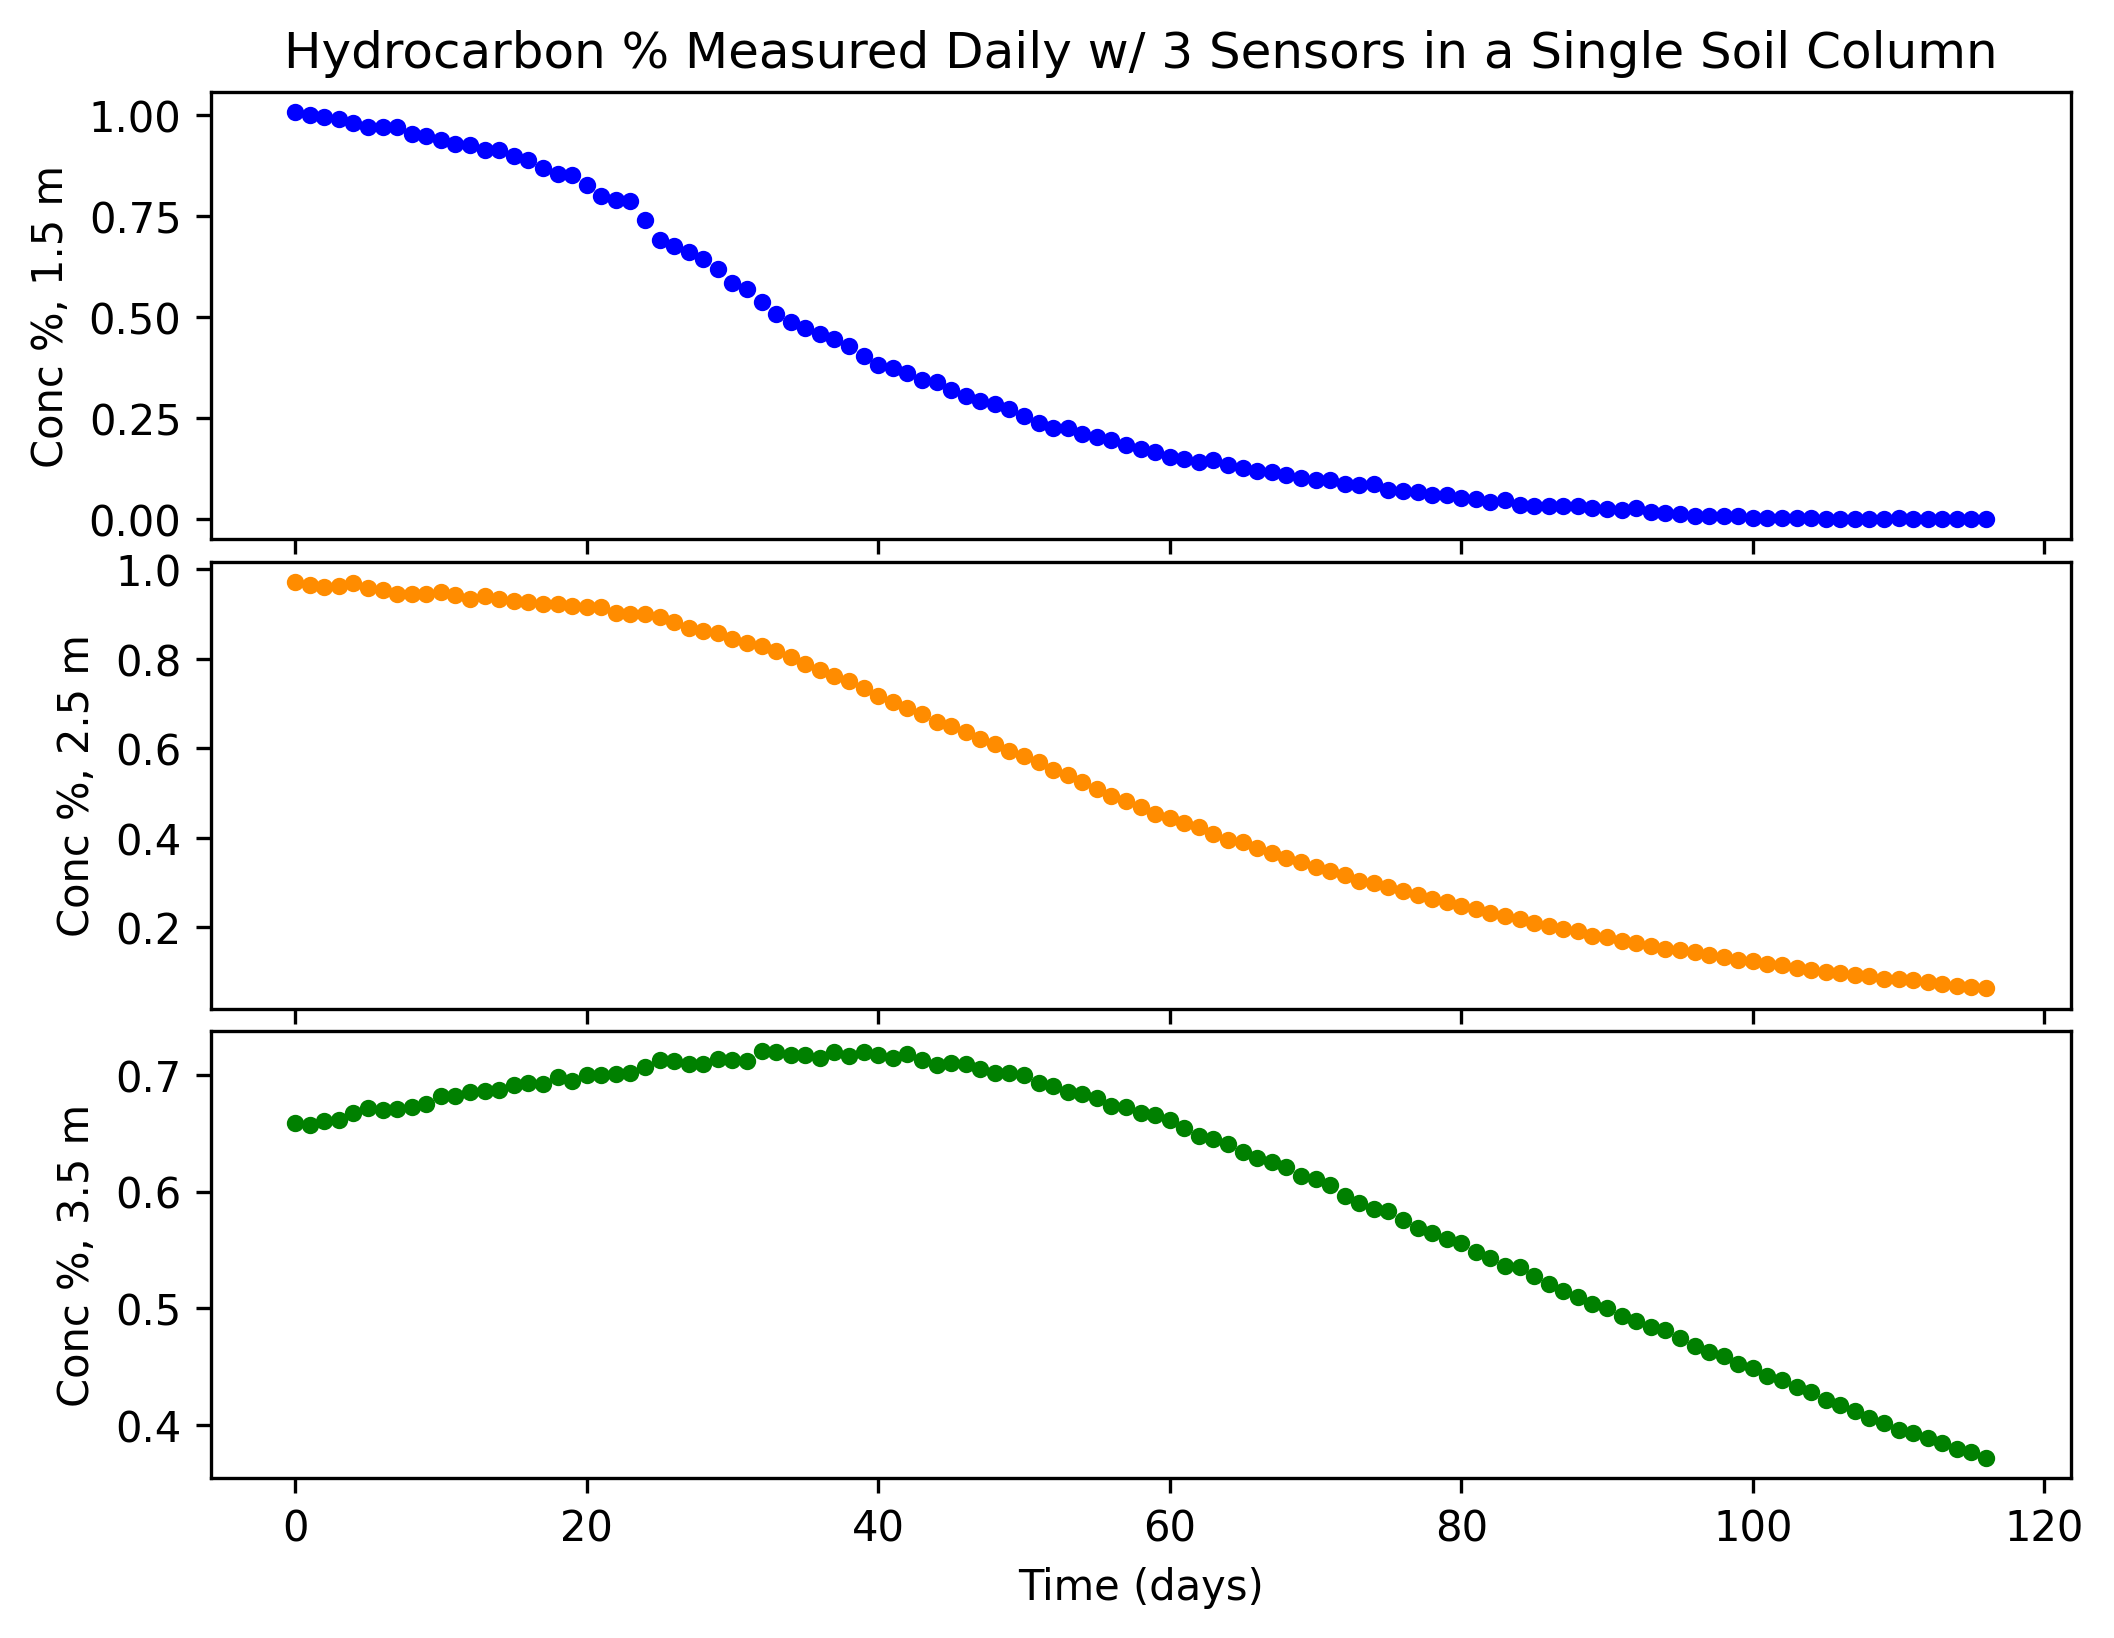
\includegraphics[height = 4in]{figures/real_measurements.png}
 \caption{A sample from the real-world dataset. The three plots depict PHC concentration as a percentage of the atmosphere over a four-month span at each of the three measurement depths. Measurements are aggregated every 12 hours.}
 \label{fig:realMeas_intro}
 \end{figure}



The duration of the time series varies considerably across samples, ranging from 30 to 250 days. This variability reflects the practical realities of field deployment. Sensors were installed and occasionally decommissioned at different times throughout the remediation process, and some units experienced extended periods of dropout due to hardware faults or adverse weather conditions. As a result, the dataset is irregular with stake locations distributed non-uniformly across the site and each location contributing multiple different lengths of observational records. These characteristics make the dataset representative of the kind of incomplete, heterogeneous data that spatial interpolation methods must contend with in real remediation settings.

A representative sample is shown in Figure~\ref{fig:realMeas_intro}, illustrating the range of behaviours observed across stake locations. Some locations exhibit a clear monotonic decline in PHC concentration consistent with active biostimulation, while others show more complex dynamics including periods of stagnation or transient increases, likely attributable to soil heterogeneity or localised variations in nutrient distribution.






\section{Synthetic Data}
\label{sec:synthetic_data}

A synthetic data sample largely mirrors the real-world data format. Each sample contains measurements at depths of 1.5~m, 2.5~m, and 3.5~m at 12-hour intervals. These properties can be varied when testing the methods under different conditions.

The synthetic data is generated from a physics-based simulation that incorporates diffusion, advection, and biodegradation of PHC concentration. The simulation operates in one dimension along the depth of the soil column, consistent with the single-stake measurement setup. 

The total simulation depth is fixed at 4.5~m that balances not extending the simulation too far past the important parts (the sensors) with a shallow estimate of the vadose zone depth in Western Canada \cite{groundWater_levels}. The individual simulation cell depth $(\Delta\distvar)$ is fixed at 0.1~m which provides sufficient granularity in the soil column while keeping computation feasible. The simulation time step $(\Delta\timevar)$ is one hour to reduce computation and is sufficient at the time scales of soil transport and bioremediation \cite{groundwater_modeling_standards}. The forward model governing contaminant concentration through time is: 



\begin{equation}
\label{eq:soil_model}
\begin{aligned}
    \conc(\locvar_i,\, \timevar + \Delta\timevar) = \; & \conc(\locvar_i,\, \timevar) \\
    & + \advecCoeff(\locvar_i)
        && \text{(Advection)} \\
    & + \biodegCoeff(\locvar_i) \cdot \conc(\locvar_i,\, \timevar)
        && \text{(Biodegradation)} \\
    & + \diffCoeff(\locvar_i) \cdot \frac{\Delta\timevar}{\Delta\distvar^{2}}
      \Bigl[
        \conc(\locvar_{i- \Delta\distvar} ,\, \timevar)
        - 2\conc(\locvar_i,\, \timevar)
        + \conc(\locvar_{i + \Delta\distvar},\, \timevar)
      \Bigr]
        && \text{(Diffusion)}
\end{aligned}
\end{equation}

\noindent
where $\conc(\locvar_i,\,\timevar)$ is the PHC concentration (\%) at depth $\locvar_i$~(m) and time $\timevar$~(hours). $\advecCoeff(\locvar_i)$ is a simplified lateral advection term ranging from $\bigl(-10^{-3},\;10^{-3}\bigr)$~\%\,hour$^{-1}$ \cite{AdvectionCoeff}. $\biodegCoeff$ is a proportional biodegradation rate representing the natural microbial breakdown of PHC in the soil, ranging from $\bigl(-10^{-3},\;10^{-3}\bigr)$~hour$^{-1}$ \cite{biodeg}. $\diffCoeff$ is the vertical diffusion coefficient governing PHC transport between neighbouring cells, ranging from $\bigl(10^{-10},\;10^{-6}\bigr)$~m$^{2}$\,hour$^{-1}$ \cite{diffcoeff, tempCoeff}. All three soil parameters are realized as vectors with one value per simulation cell. Five pilot-point values are drawn from the distributions shown in Figure~\ref{fig:sim_param_dist} and assigned to depths of 0, 1.1, 2.2, 3.3, and 4.5~m; all intermediate cell values are obtained by interpolation.


\subsection{Soil Parameterization}

Once the parameter vectors are constructed, the initial PHC concentration $\conc(\locvar,\,0)$ and boundary conditions must be specified for all cells.

Four boundary condition scenarios are used to generate the simulated dataset. A PHC source at both the top and bottom of the soil column, at the top only, at the bottom only, and at neither. These cases represent the principal real-world configurations in which PHC originates from the surface, the water table, both, or neither \cite{hydrocarbon_in_soil_old,PHC_in_soil_newer}. Source boundary concentrations are drawn from a normal distribution with a mean of 3\% and a standard deviation of 0.5\%; all other initial PHC concentrations are drawn with a mean of 0.12\% and a standard deviation of 0.04\%, with a lower threshold of 0\%. These values are derived from the real-world data in Section~\ref{sec:real_data} and from the literature~\cite{biodeg, oil_conc_soil}. As with the soil parameters, values are assigned at pilot-point locations and interpolated across all remaining cells.


\begin{figure}[!h]
    \centering
    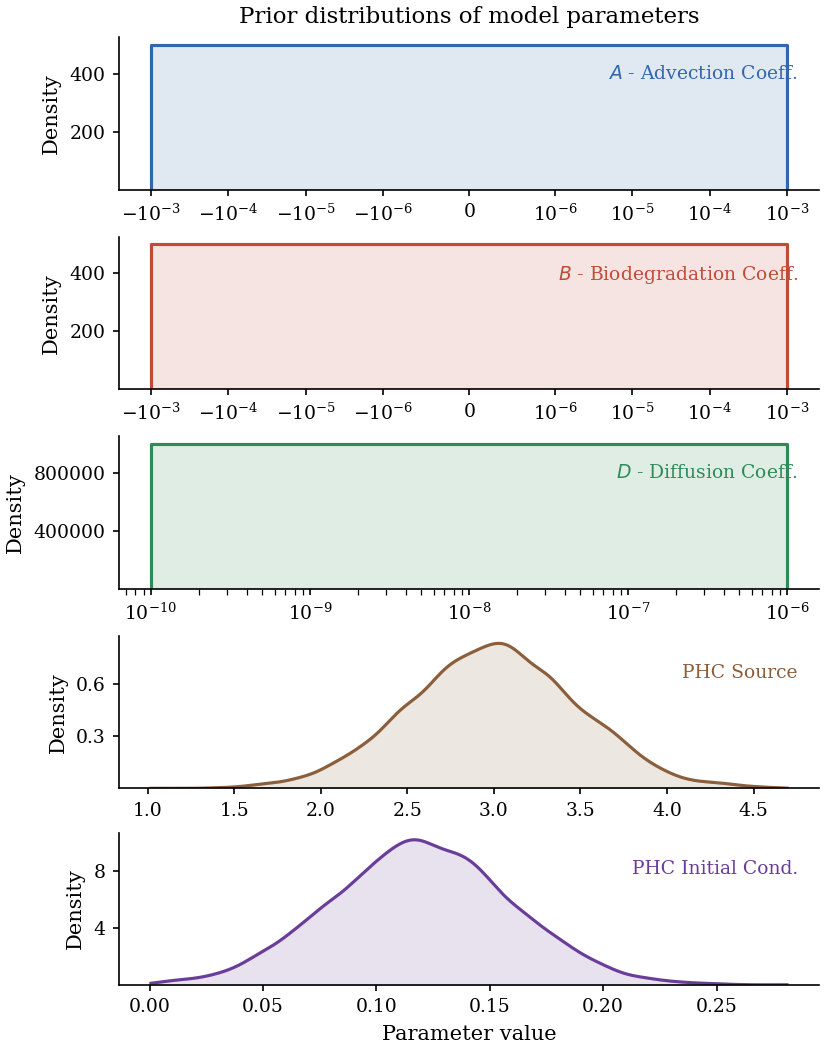
\includegraphics[height=5in]{figures/param_dist.png}
    \caption{Sample distributions of the soil parameters, PHC source boundary conditions, and PHC initial values.}
    \label{fig:sim_param_dist}
\end{figure}

\subsection{Parameter Regularizaton}

An important step in both the random drawing of parameters and the update phase of parameter estimation is regularization. Normalising all parameters to the range $[0, 1]$ during the update phase improves numerical stability and simplifies the drawing of uniform samples~\cite{pestManual, regularization}.

The boundary and initial conditions of PHC concentration are straightforward. All values are mapped linearly from their physical range of $[0, 4]$ to $[0, 1]$. The regularization of the boundary conditions and the initial conditions of PHC are quite straightforward. All of them are transformed linearly from 0-4 to 0-1. The diffusion coefficient requires a different treatment because it spans four orders of magnitude. The diffusion parameter $\diffCoeff \in [10^{-10},\, 10^{-6}]$~m$^2$/s is mapped to a normalised variable $\tilde{\diffCoeff} \in [0, 1]$ via a log-linear transformation. The forward transformation from $\tilde{\diffCoeff}$ to $\diffCoeff$ is

\begin{equation}
    \diffCoeff(\tilde{\diffCoeff}) = 10^{-10 + 4\tilde{\diffCoeff}},
\end{equation}

and the inverse is 

\begin{equation}
    \tilde{\diffCoeff}(\diffCoeff) = \frac{\log_{10}(\diffCoeff) + 10}{4}.
\end{equation}

This normalization ensures that equal increments in $\tilde{\diffCoeff}$ correspond to equal multiplicative steps in $\diffCoeff$, preserving sensitivity across the full range of the parameter space.

The advection coefficient $\advecCoeff$ and biodegradation coefficient $\biodegCoeff$ are signed quantities spanning $[-10^{-3},\, 10^{-3}]$. The following derivation uses $\advecCoeff$ for notational convenience, but both parameters employ the same transformation. Since a purely logarithmic mapping is undefined near zero, a piecewise transformation is used: a linear core region of half-width $\advecCoeff_0 = 10^{-6}$ and a logarithmic outer region extending to $|\advecCoeff| = \advecCoeff_1 = 10^{-3}$. The normalised variable $\tilde{\advecCoeff} \in [0, 1]$ is related to an intermediate variable $v = 2\tilde{\advecCoeff} - 1 \in [-1, 1]$. The forward transformation from $v$ to $\advecCoeff$ is

\begin{equation}
    \advecCoeff(v) =
    \begin{cases}
        \displaystyle \advecCoeff_0 \frac{v}{v_0}, & |v| \leq v_0, \\[10pt]
        \displaystyle \operatorname{sgn}(v)\, \advecCoeff_0 \left(\frac{\advecCoeff_1}{\advecCoeff_0}\right)^{\!\frac{|v| - v_0}{1 - v_0}}, & |v| > v_0,
    \end{cases}
\end{equation}

with $v_0 = 0.1$. The inverse transformation from $\advecCoeff$ to $\tilde{\advecCoeff}$ is recovered by first computing

\begin{equation}
    v(\advecCoeff) =
    \begin{cases}
        \displaystyle v_0 \frac{\advecCoeff}{\advecCoeff_0}, & |\advecCoeff| \leq \advecCoeff_0, \\[10pt]
        \displaystyle \operatorname{sgn}(\advecCoeff) \left( v_0 + (1 - v_0)\frac{\ln(|\advecCoeff|/\advecCoeff_0)}{\ln(\advecCoeff_1/\advecCoeff_0)} \right), & |\advecCoeff| > \advecCoeff_0,
    \end{cases}
\end{equation}

\noindent
and then applying $\tilde{\advecCoeff} = (v + 1)/2$. The linear core ensures smooth, symmetric behaviour near zero, while the logarithmic outer region preserves sensitivity across the several orders of magnitude spanned by $|\advecCoeff|$.




\subsection{Visualization}
With all soil parameters and initial conditions drawn from the distributions described above, each realisation constitutes a single sample in the simulated dataset. Example plots are shown in Figure~\ref{fig:sim_ex}, illustrating the format of visualisations used throughout the results section to compare model outputs.


\begin{figure}[H]
    \centering
    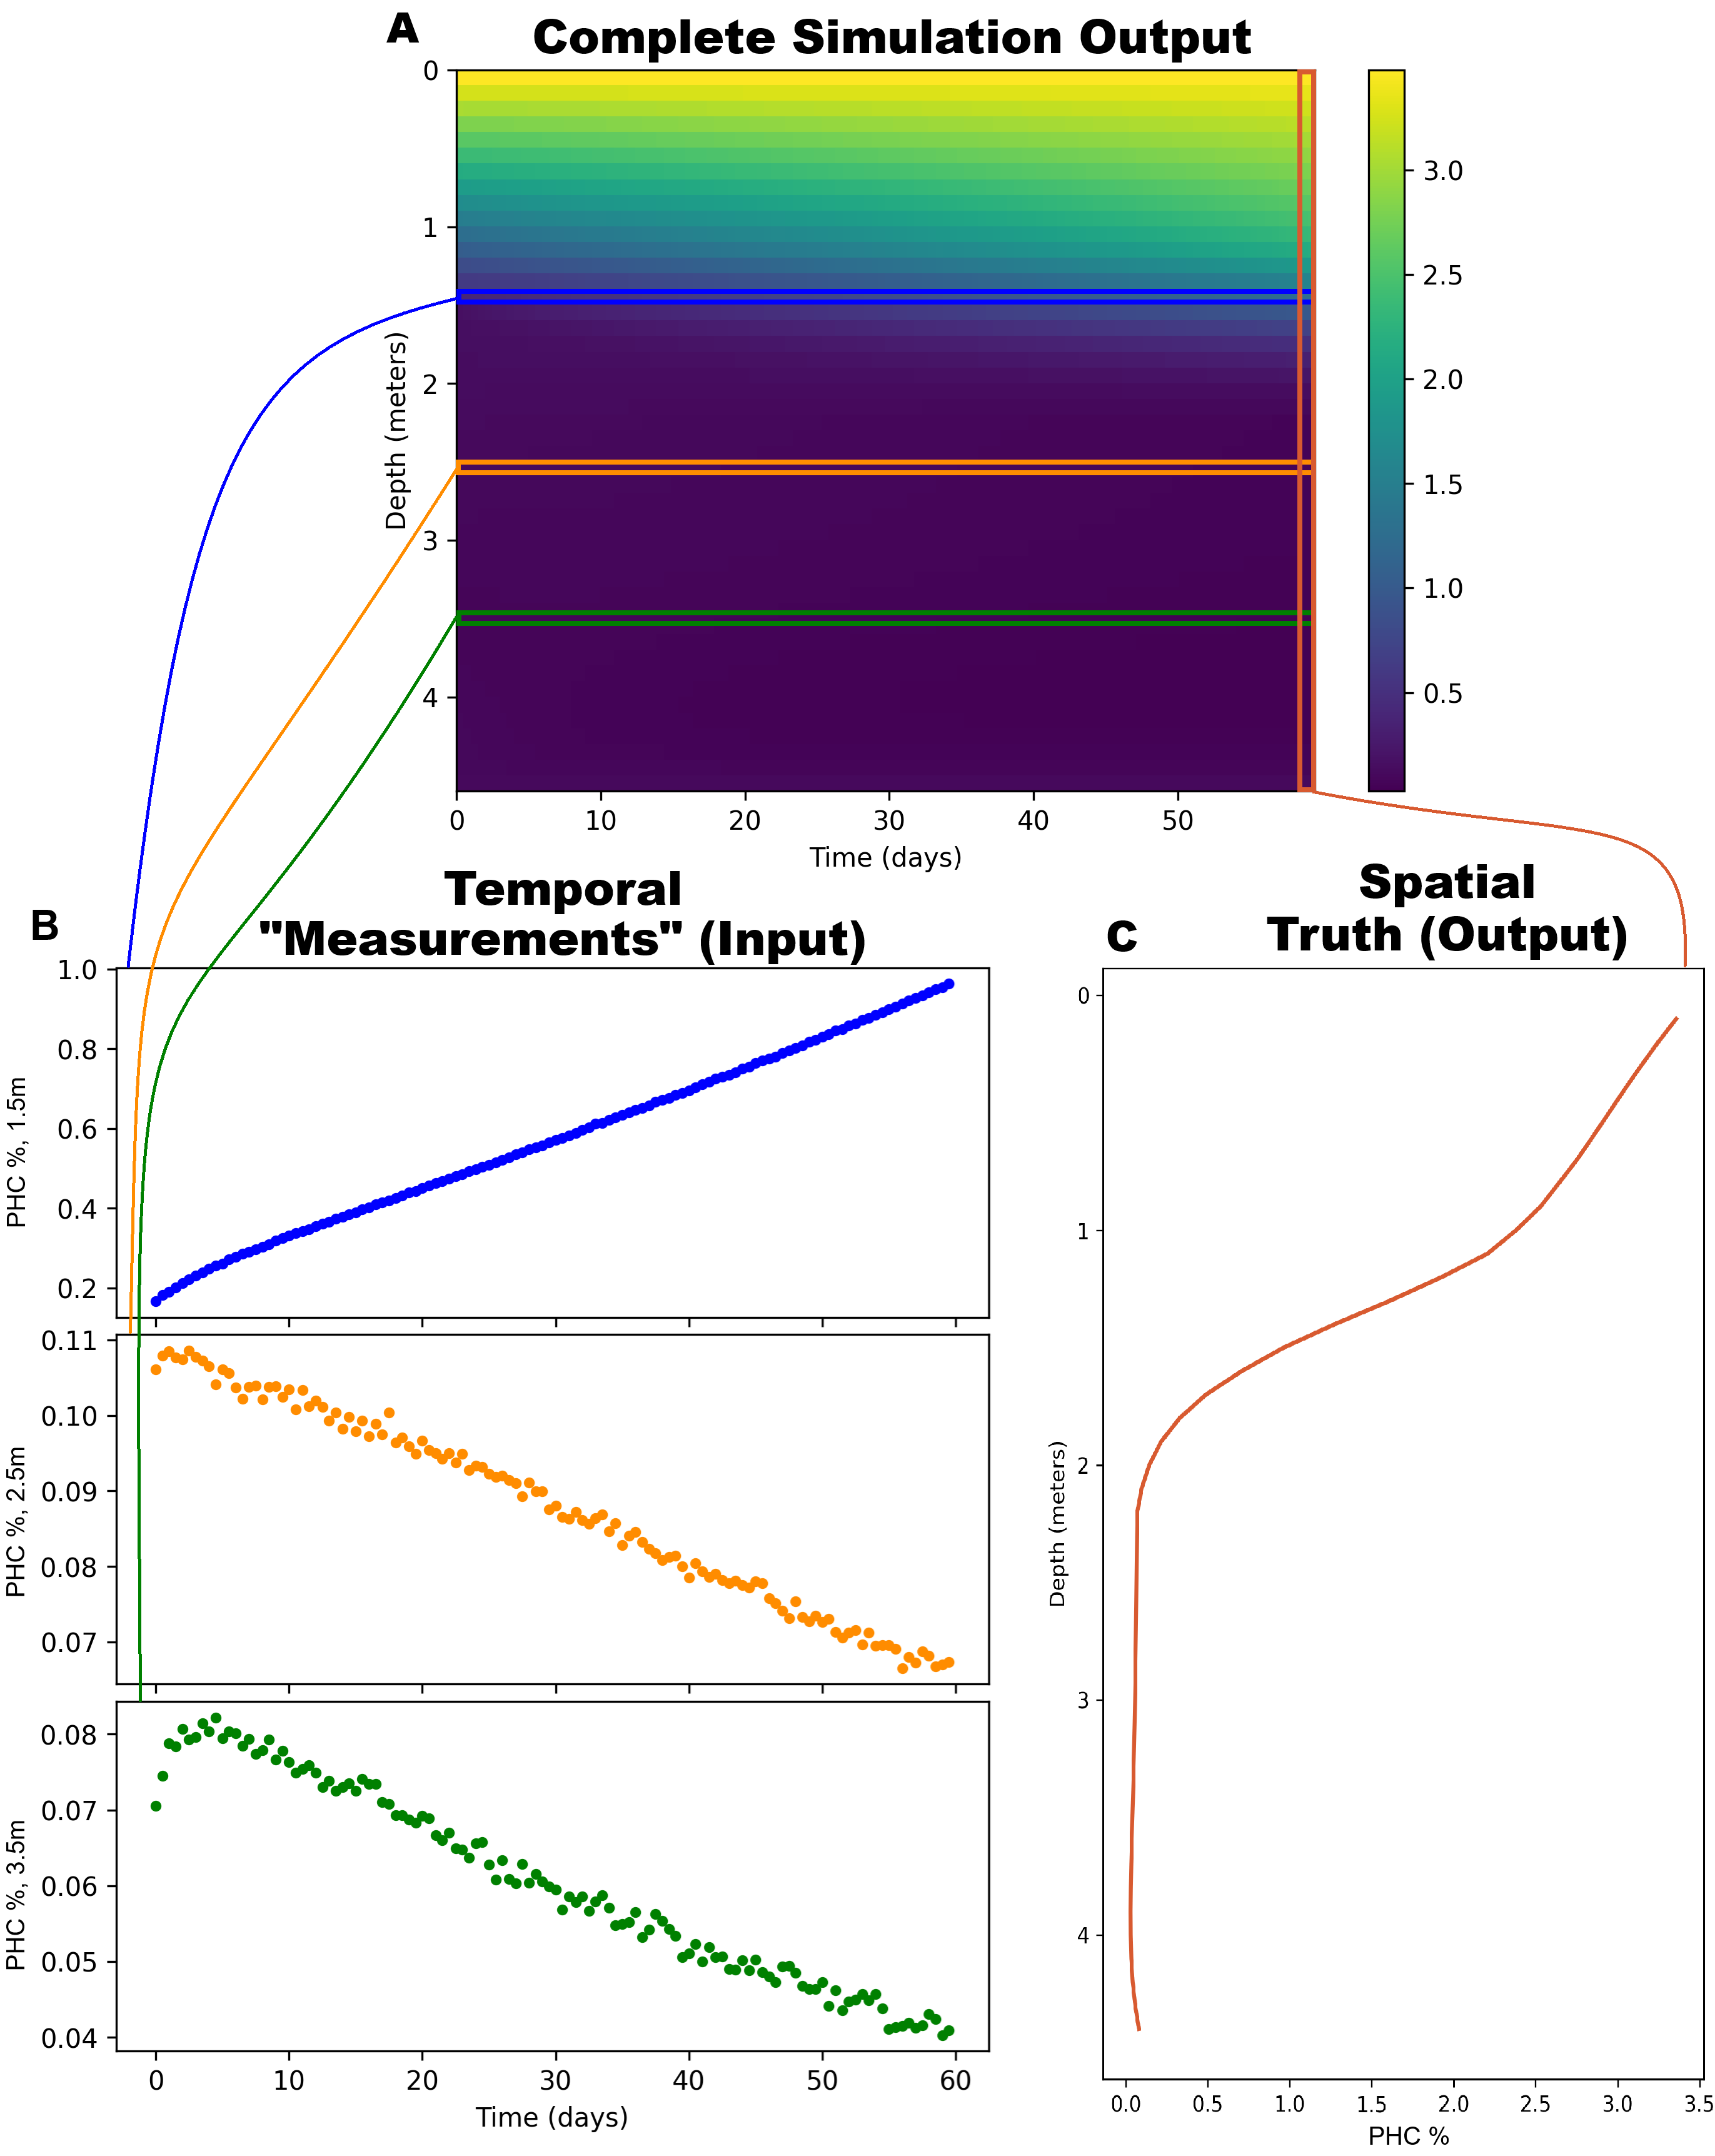
\includegraphics[width=6in]{figures/sim_data_sample.png}
    \caption{A sample of simulated data. (a) PHC concentration through time across all simulated cells. Cell size is 0.1~m deep and 12 hours wide. (b) Sensor-format time series, equivalent to the real-world example in Figure~\ref{fig:realMeas_intro}. This serves as the input to the spatial interpolation methods. (c) Spatial distribution of the contaminant plume at the end of the simulation. This is the output the methods aim to reconstruct.}
    \label{fig:sim_ex}
\end{figure}

Figure~\ref{fig:sim_ex} illustrates how these three panels relate to one another for a single realisation. In (a), a surface-source synthetic sample is shown, with time on the x-axis and soil depth on the y-axis; colour represents the PHC concentration at each depth and time. The horizontal boxes mark the depths of the three simulated sensors, at 1.5~m, 2.5~m, and 3.5~m, whose corresponding time series are shown in (b). The vertical box marks the PHC concentration at the $\nSampTime^{th}$ time step, which is used as the spatial ground truth in (c). Panel (b) shows the temporal evolution of PHC at each of the three sensor depths; this is the input the methods receive in order to predict the ground truth in (c). Finally, (c) shows the spatial distribution of PHC concentration with depth at the final time step $\nSampTime$, which is the ground truth that the methods aim to reconstruct from the sparse measurements in (b).

\section{Synthetic Variations}

The preceding sections describe the fundamental simulation model: the forward physics governing PHC transport and biodegradation, the distributions from which soil parameters and boundary conditions are drawn, and the regularization scheme used to constrain them. This model, run under its default configuration, is used to generate the base simulated dataset of $\valsize$ samples, distributed equally among the four source configurations: both, bottom-only, top-only, and neither. The remainder of this section departs from this fundamental model to describe a set of controlled experimental manipulations applied to the base dataset. Rather than altering the underlying physics, these manipulations degrade or restructure the sensor measurements sampled from it, in order to evaluate each method under a variety of conditions representative of real-world deployment. The following subsections describe each manipulation in turn: measurement noise, number of sensors, soil parameter noise, measurement frequency, and sensor dropout.

\subsection{Measurement Noise}
Gaussian noise is added to the sensor measurements to simulate real-world measurement error. Two noise levels are considered: a standard deviation of 0.001\% and a standard deviation of 0.01\%. The lower value matches the noise floor recorded by the real sensors. The higher value represents a more extreme case in which small PHC concentrations become difficult to discern and is potential failure mode in certain cases. 

\begin{figure}[H]
    \centering
    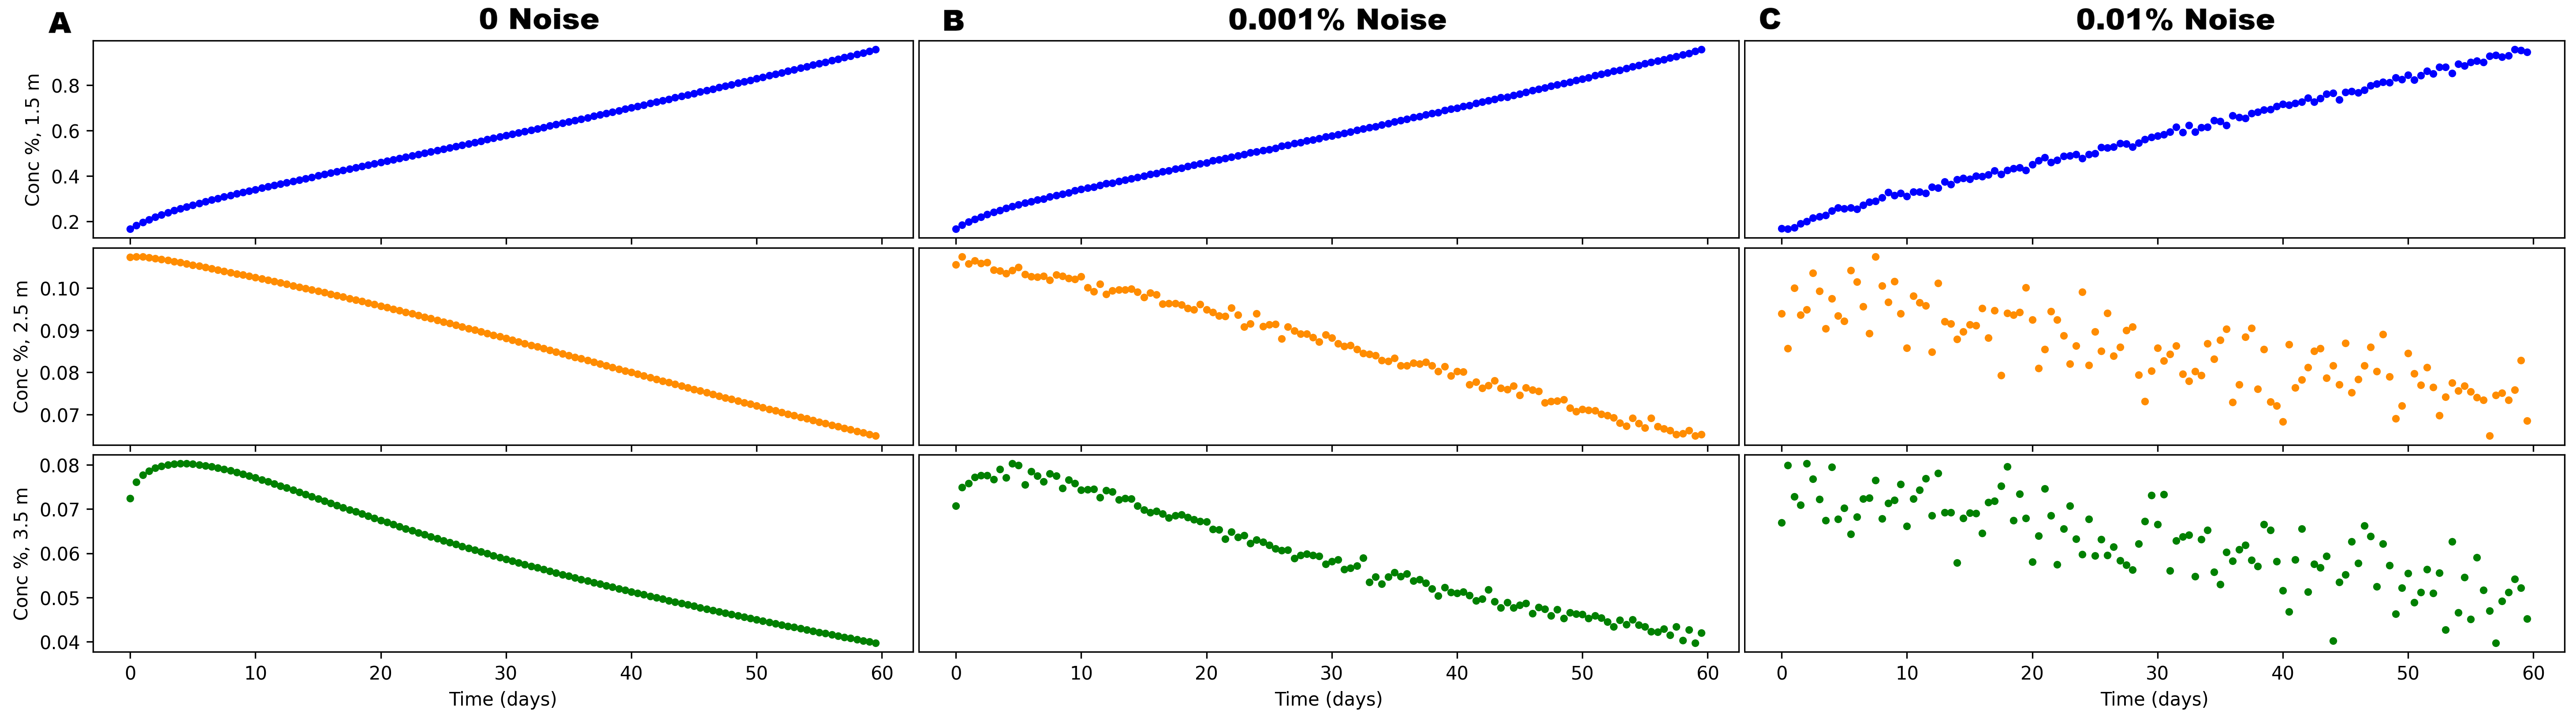
\includegraphics[width=6.5in]{figures/meas_noise.png}
    \caption{(A) The base case with no added noise. (B) and (C) show normally distributed noise with standard deviations of 0.001\% and 0.01\%, respectively.}
    \label{fig:sim_meas_noise}
\end{figure}

With the variation of measurement noise to the dataset, the interpolation methods are evaluated on their susceptibility to noisy measurements affecting their prediction. Both noise levels are applied to all \valsize~samples to produce two additional test datasets, evaluated in Section~\ref{sec:res_measNoise}.

\subsection{Number of Sensors}
The standard configuration uses three sensors per stake, consistent with the real-world setup, at depths of 1.5, 2.5, and 3.5~m. To assess the effect of sensor count on interpolation quality, configurations with 1, 2, and 4 sensors were also tested.

\textcolor{red}{What is the purpose of this figure?}
\begin{figure}[H]
    \centering
    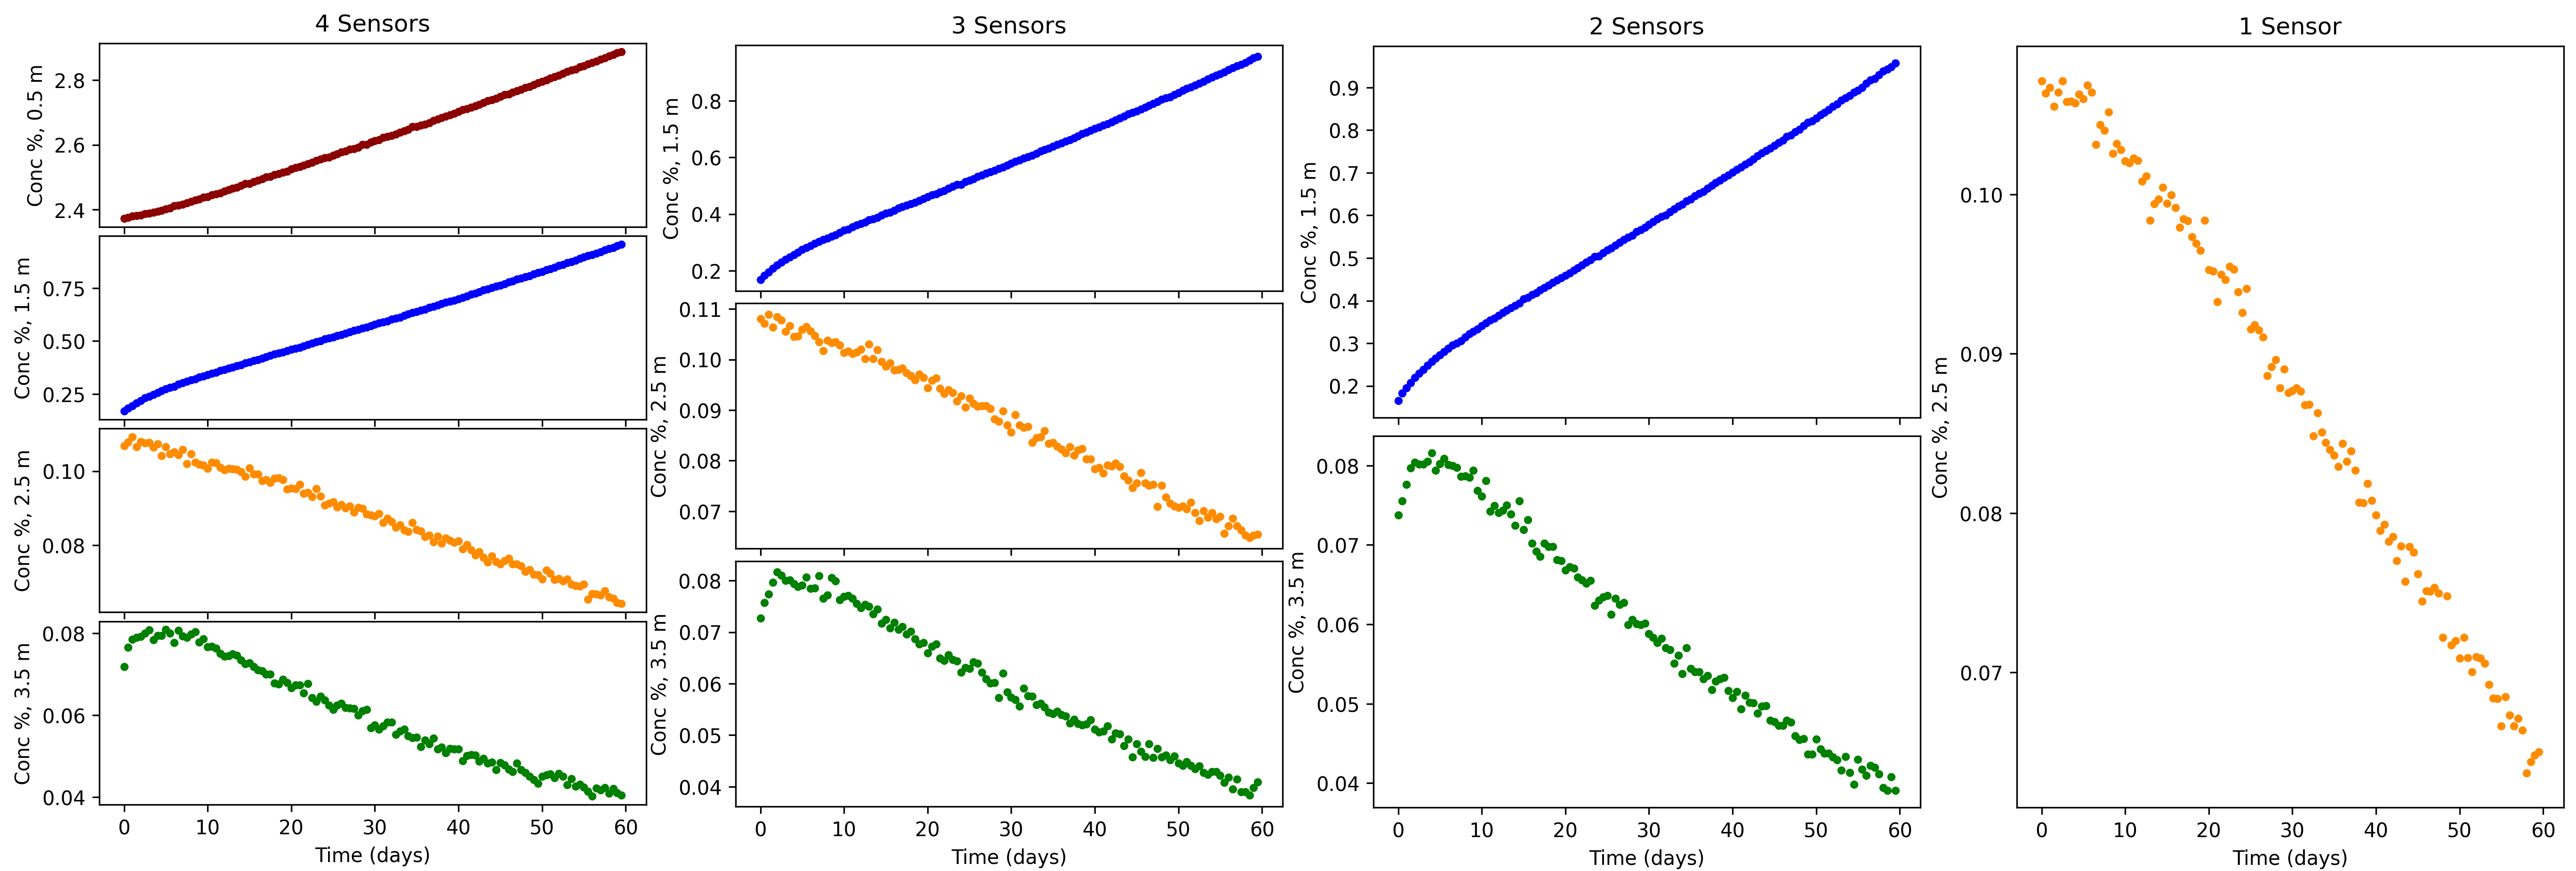
\includegraphics[width=6in]{figures/nSens.png}
    \caption{Sensor inputs for configurations ranging from 4 sensors (left) to 1 sensor (right), illustrating what each method receives as input.}
    \label{fig:sim_num_sens}
\end{figure}

Modifying the number of sensors serves three purposes. First, it helps determine the relative importance of each sensor, for example, which sensor contributes most to the spatial reconstruction. Second, it evaluates whether additional sensors provide valuable information or are largely redundant. Third, it compares each method's ability to exploit additional spatial information against its ability to cope with reduced spatial information, testing performance at both ends of the sensor-count range. As the number of sensors decreases, the methods receive less information about the spatial extent of the plume and lose visibility of the boundary conditions, which is expected to degrade the quality of spatial reconstruction. Conversely, with four sensors, the methods are expected to improve their spatial reconstruction due to the increased spatial resolution provided to them.

\subsection{Soil Parameter Noise}
The role of pilot points is central to understanding this variation. The parameter vector $\hat{\param}_0$ includes the initial PHC concentration $\conc_0$, the soil parameters $\advecCoeff$, $\biodegCoeff$, and $\diffCoeff$, and the top and bottom boundary conditions. The boundary conditions are drawn directly from the distributions in Figure~\ref{fig:sim_param_dist} according to the source configuration. The soil parameters and initial conditions, however, are not drawn independently for each of the 44 simulation cells (doing so would produce unrealistically heterogeneous soil). Instead, $\npp$ pilot points (typically 3--10) are drawn and distributed uniformly through the depth. All intermediate cell values are then obtained by interpolation. For dataset generation, the number of pilot points is fixed at 5. During interpolation, additional noise can be introduced into the pilot-point values to increase soil heterogeneity. Two levels are tested: 0.01 and 0.1, corresponding to 1\% and 10\% of the normalised parameter range, respectively.

\begin{figure}[H]
    \centering
    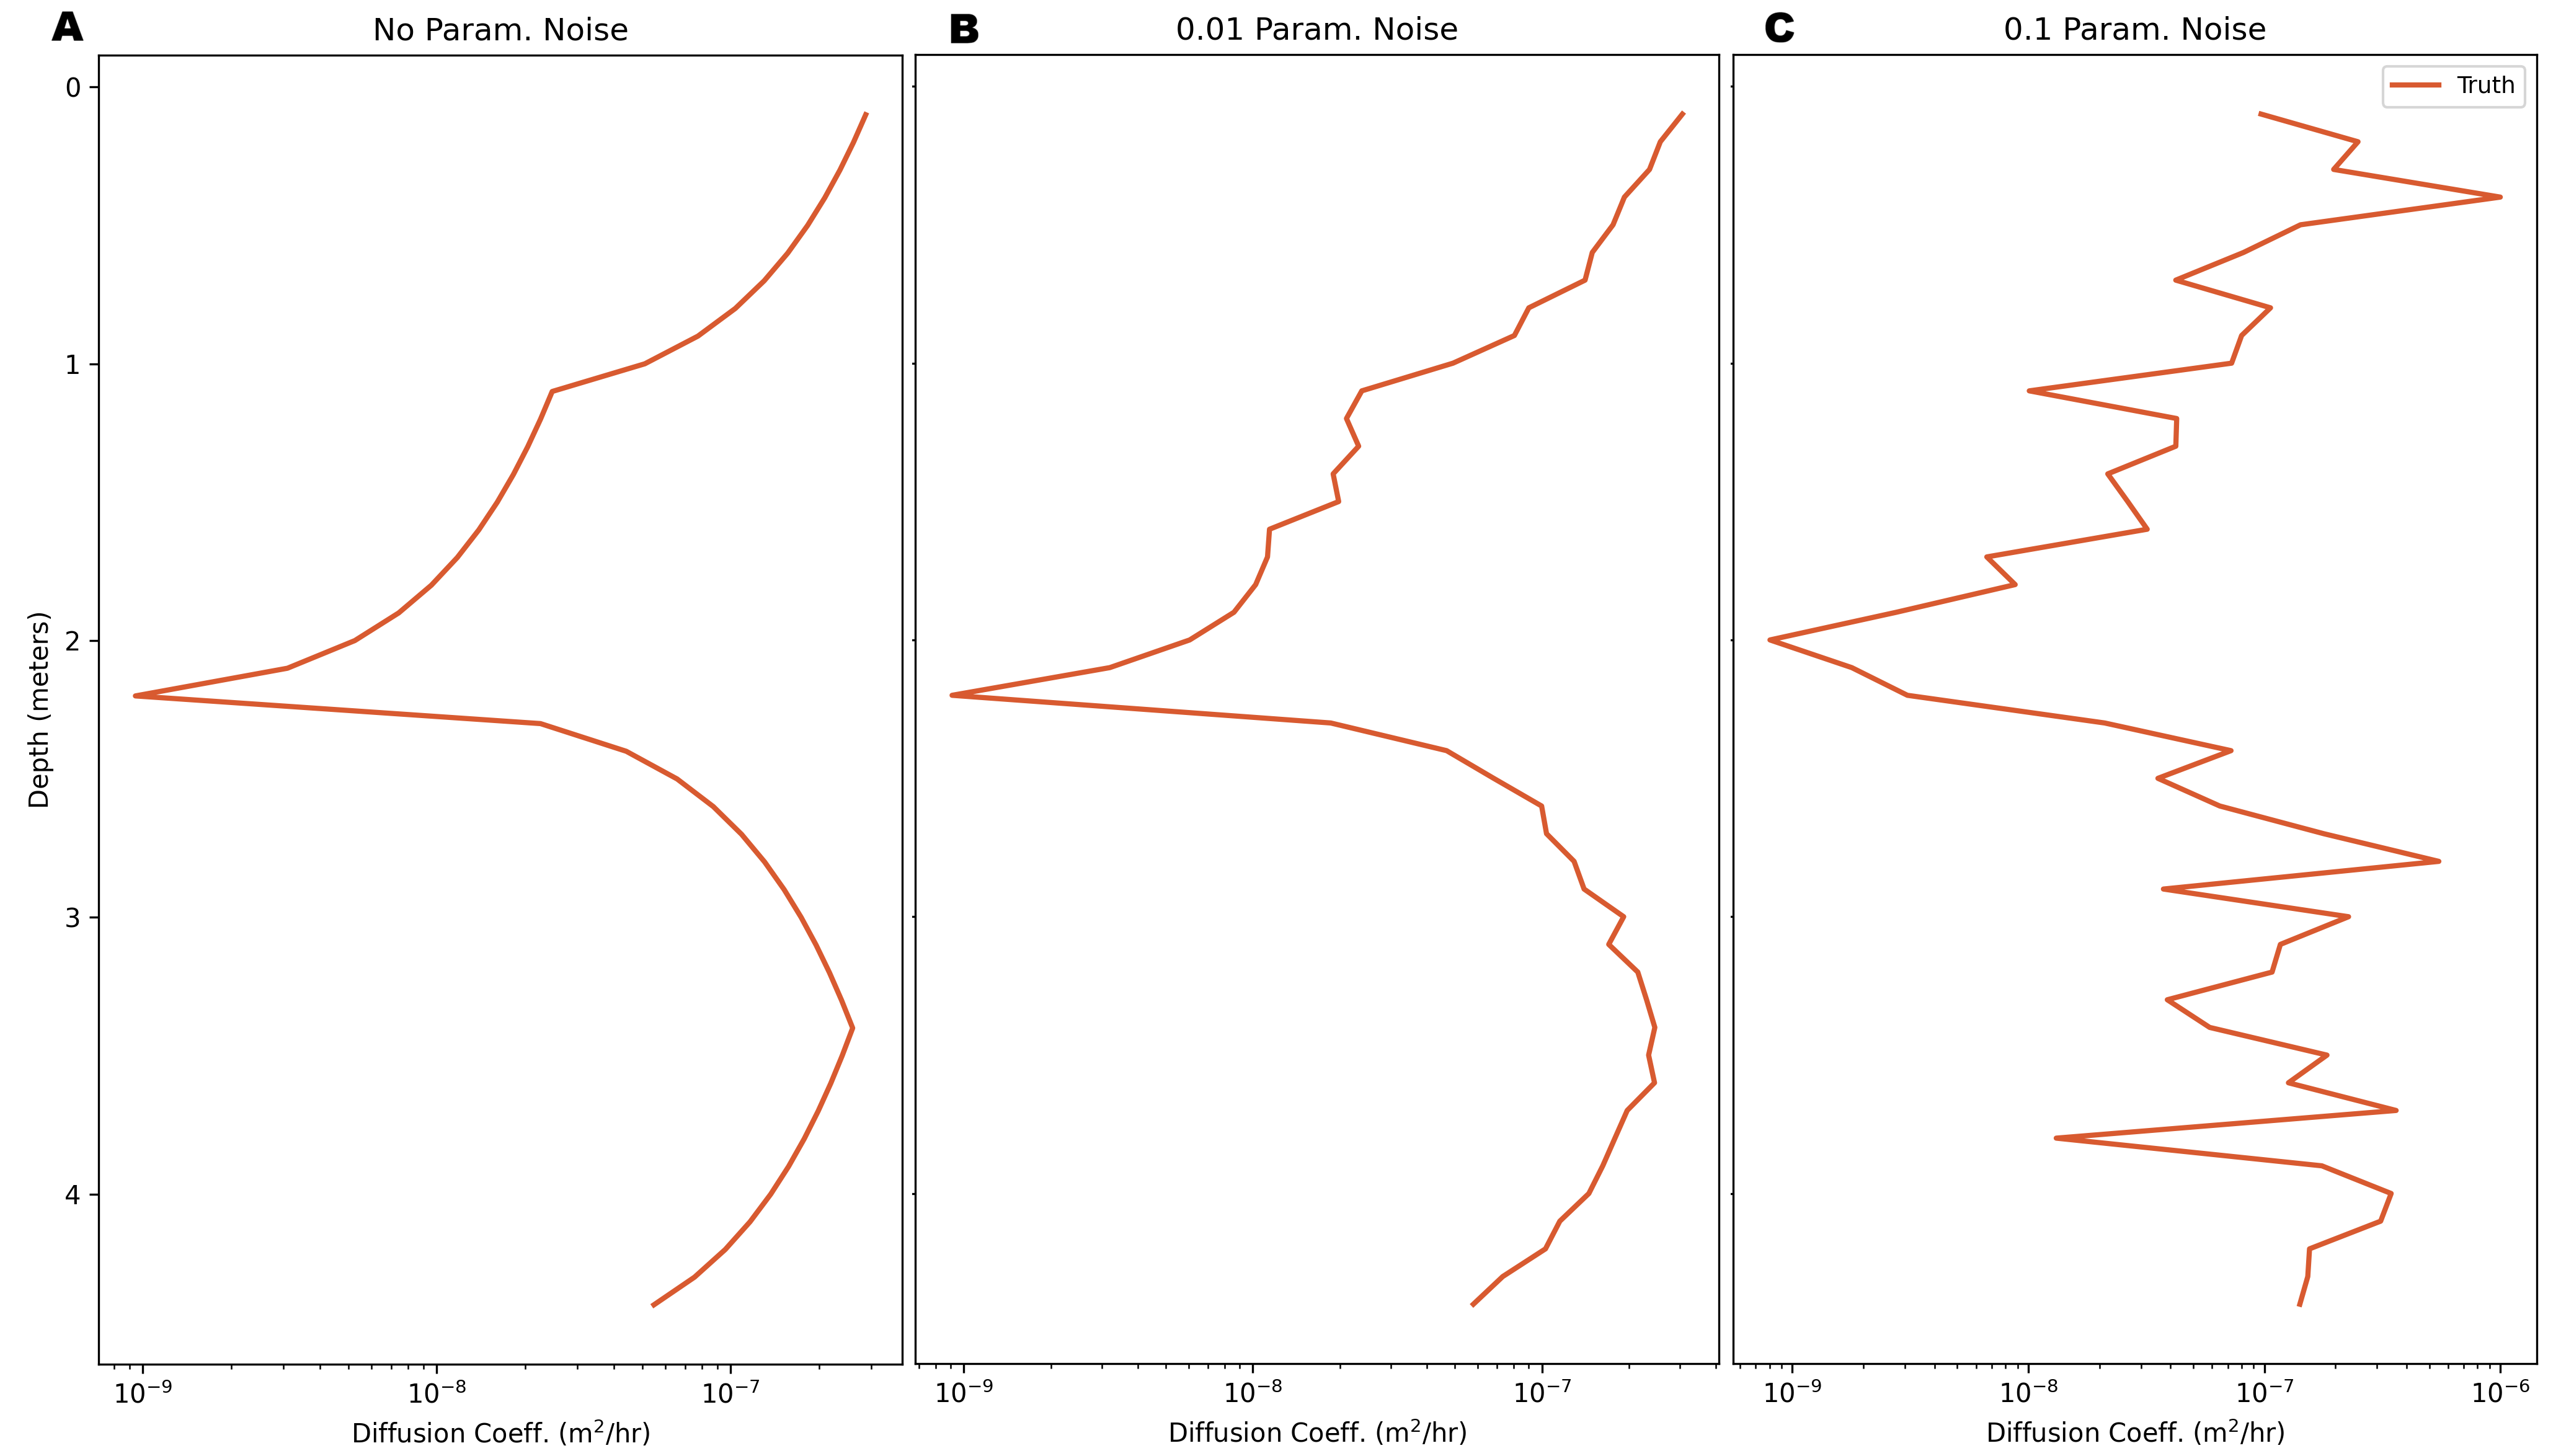
\includegraphics[width=6in]{figures/parNoise.png}
    \caption{Distribution of the diffusion coefficient through depth for a single sample. (a) No parameter noise, resulting from five randomly drawn pilot-point values. (b) Noise of 0.01 added in normalised space. (c) Noise of 0.1 added.}
    \label{fig:sim_param_noise}
\end{figure}

Figure~\ref{fig:sim_param_noise} illustrates how the diffusion coefficient distribution with depth changes as noise is added to the pilot-point values. In (a), the base diffusion coefficient is shown with depth, emulating heterogeneous soil composition in which properties vary smoothly with depth. In (b), noise of 0.01 is added to the regularised coefficient, producing slightly more heterogeneous soil; the underlying distribution with depth is still largely preserved despite the added noise. Finally, in (c), noise of 0.1 is added, and the original distribution is barely discernible beneath the resulting variability. This variation is intended to test the interpolation methods under highly heterogeneous soil conditions, representing something of a worst-case scenario.

Varying the soil parameter noise tests the interpolation methods' ability to handle highly heterogeneous soil properties, which are common in real-world settings but poorly captured by the pilot-point representation used to generate the base dataset. This manipulation is a reasonable stress test precisely because it targets the simplifying assumption that the parameter estimation methods rely on an internal physics-based soil model that is fit against a small number of pilot points, and increasing noise pushes the true soil parameters further from what such a model can represent. We aim to evaluate at what point the parameter estimation methods begin to fail as a result, since their internal soil models are unable to replicate increasingly noisy, fine-grained soil properties. The distance-based interpolators, by contrast, make no such structural assumption about the soil and may therefore prove more robust in the noisiest cases, potentially outperforming the parameter estimation methods despite their weaker performance elsewhere.

\subsection{Measurement Frequency}

This variation examines only the effect of increasing measurement frequency; decreased frequency is instead addressed by the sensor dropout experiments in Section~\ref{sec:exp_set_sensor_dropout}. The baseline measurement interval is 12 hours, consistent with the real-world data. A reduced interval of 4 hours is tested to determine whether the additional temporal resolution improves spatial reconstruction quality, despite the corresponding reduction in the number of raw 30-minute readings averaged into each measurement, which increases measurement noise. Intervals of up to one week were also tested, but produced results that overlapped substantially with the sensor dropout experiments and were not pursued further.

\begin{figure}[H]
    \centering
    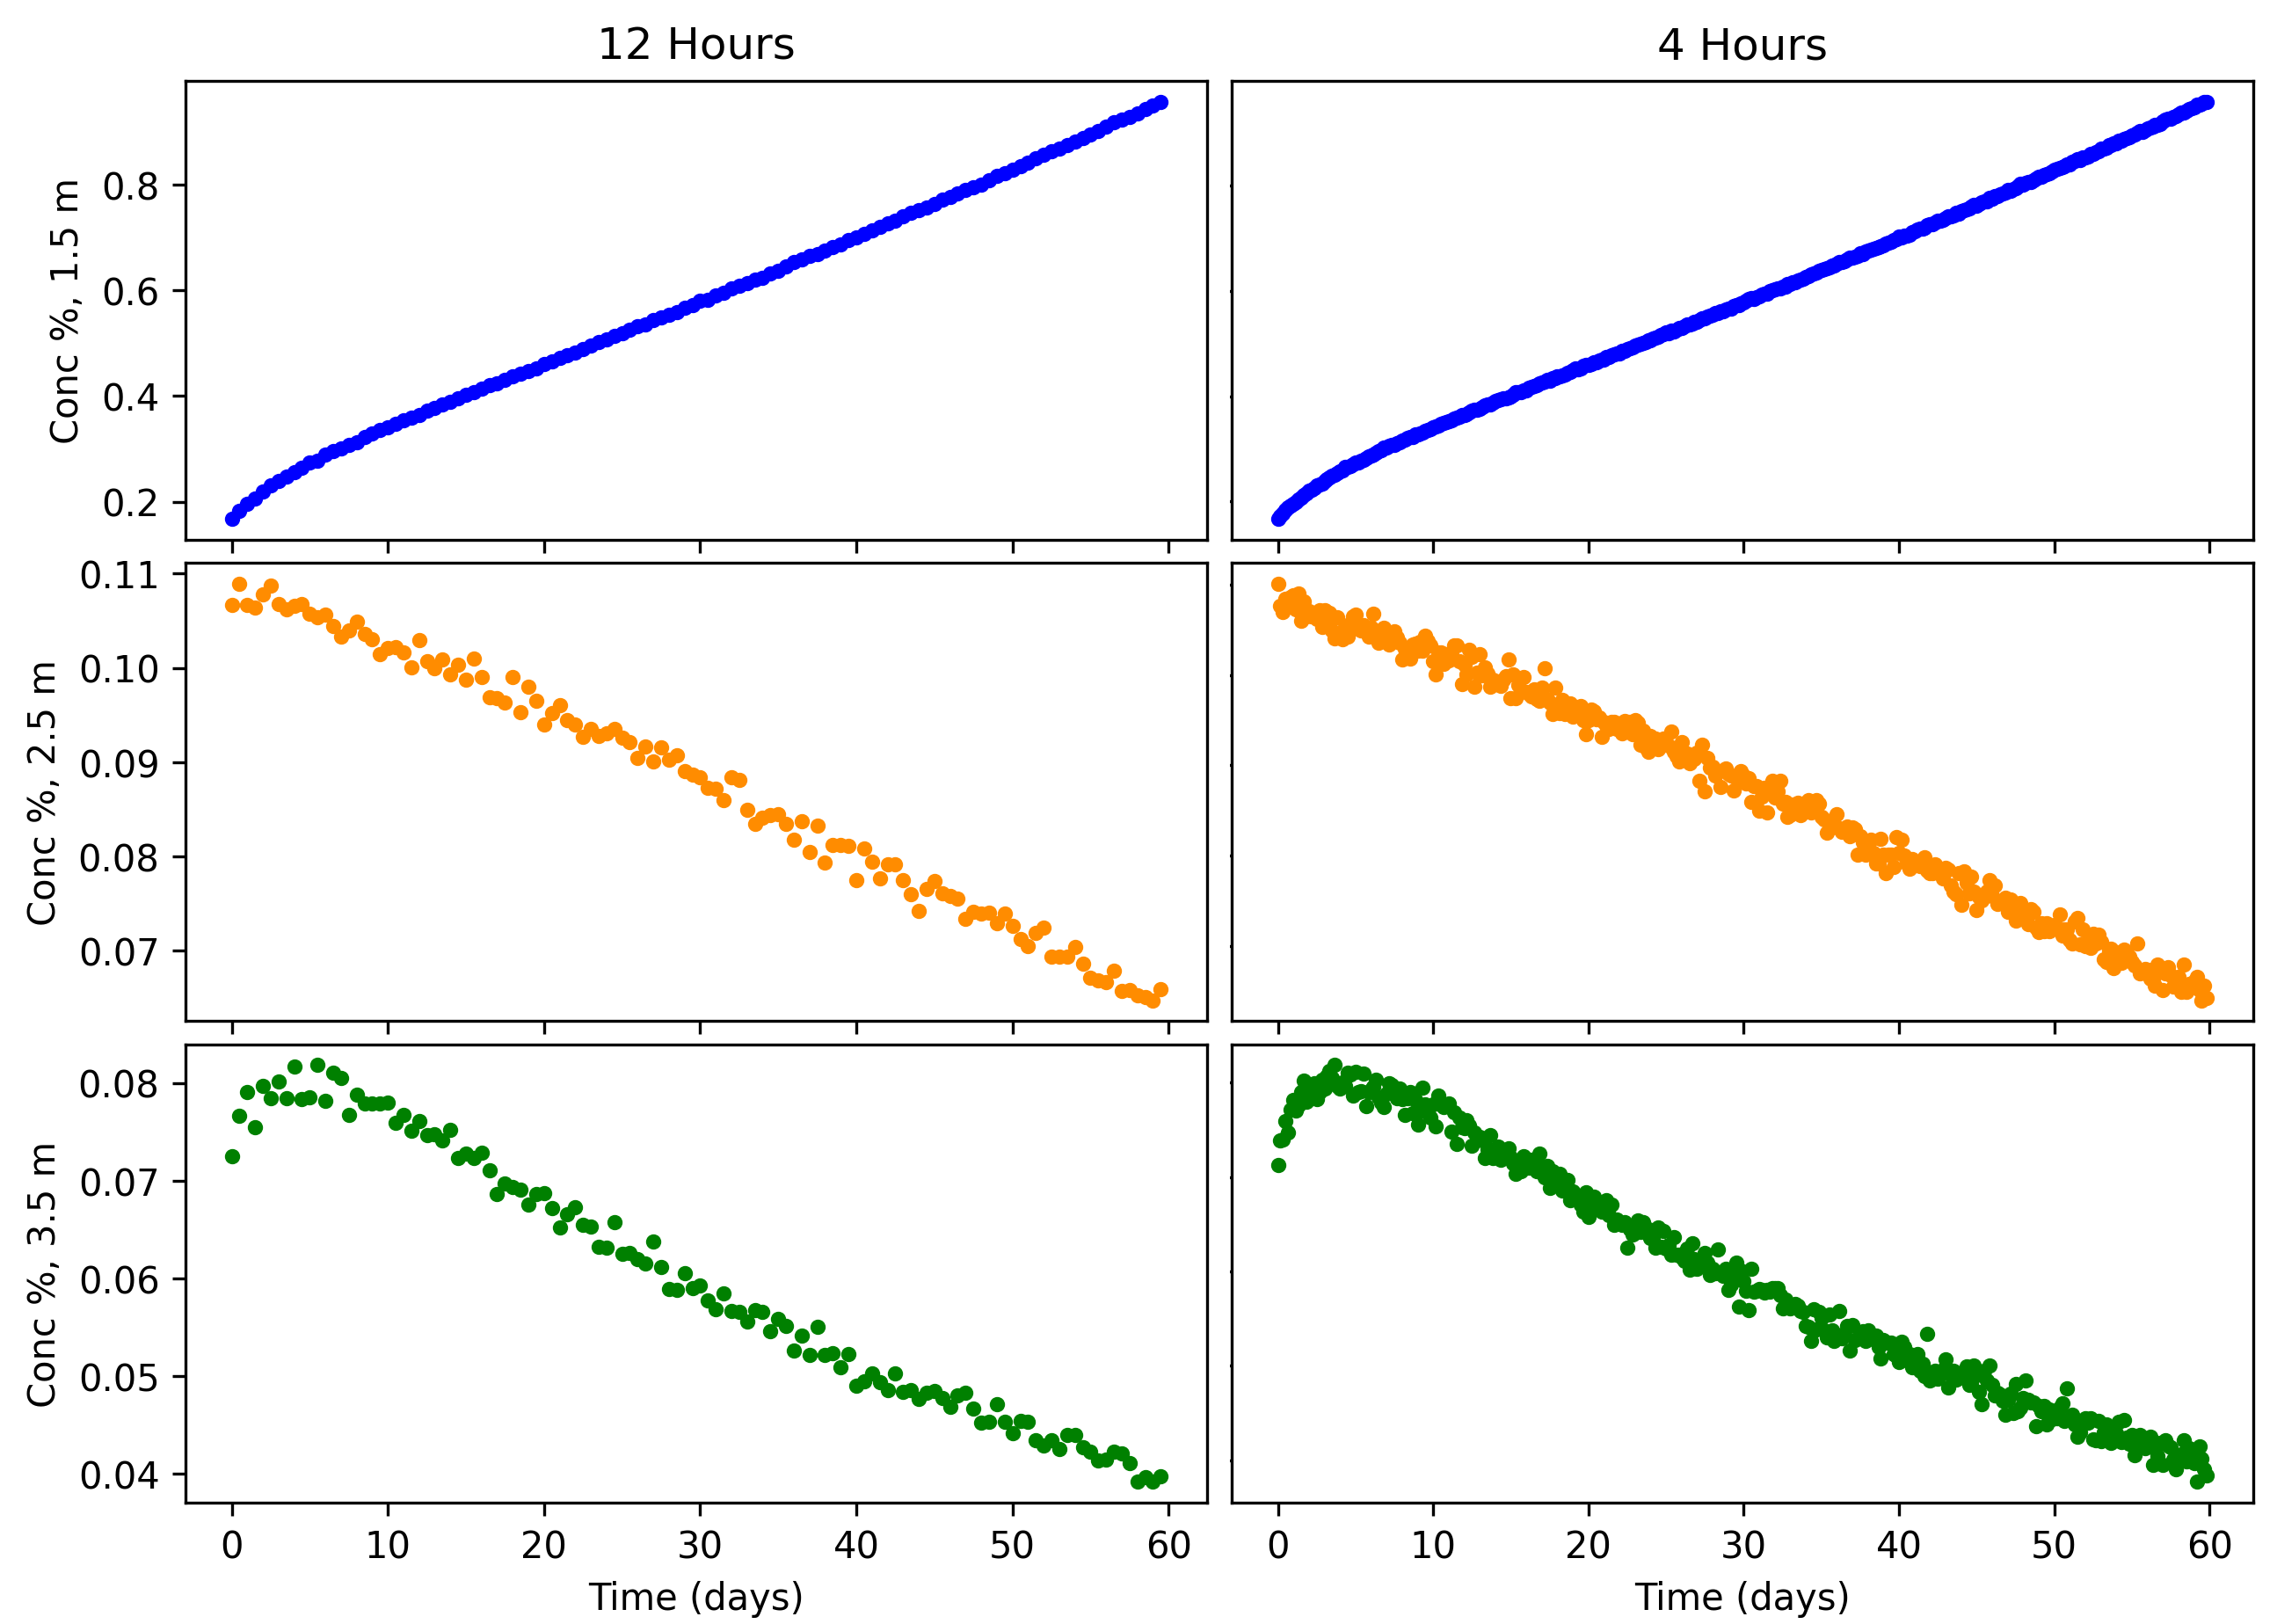
\includegraphics[height=4in]{figures/measFreq.png}
    \caption{Comparison of the default 12-hour measurement interval and the 4-hour interval.}
    \label{fig:sim_measFreq}
\end{figure}

Evaluating the models under increased measurement frequency has practical value: it informs field workers whether more frequent sampling is worth the added cost, or whether the existing 12-hour interval is already sufficient. This is a reasonable manipulation to test since the real-world sensors already sample at 30-minute intervals before aggregation, so a 4-hour interval requires no change to the underlying hardware. It also lets us evaluate whether certain methods exploit the additional temporal information better than others; the parameter estimation methods, which fit against the full temporal record, may benefit more from denser sampling than the distance-based methods, which do not model temporal dynamics. Expectations for improvement are modest, since the 12-hour baseline already provides a comparatively dense temporal record, but this is still an important check before recommending against increased sampling frequency in practice.

\subsection{Sensor Dropout}
\label{sec:exp_set_sensor_dropout}
Several dropout scenarios are evaluated to assess robustness to missing data. Salt-and-pepper noise is used to randomly remove 10\% and 50\% of temporal measurements. A complete blackout scenario, in which 50\% of the temporal data is removed as a contiguous block, is also tested to simulate sustained sensor outages common in field deployments.

\begin{figure}[H]
    \centering
    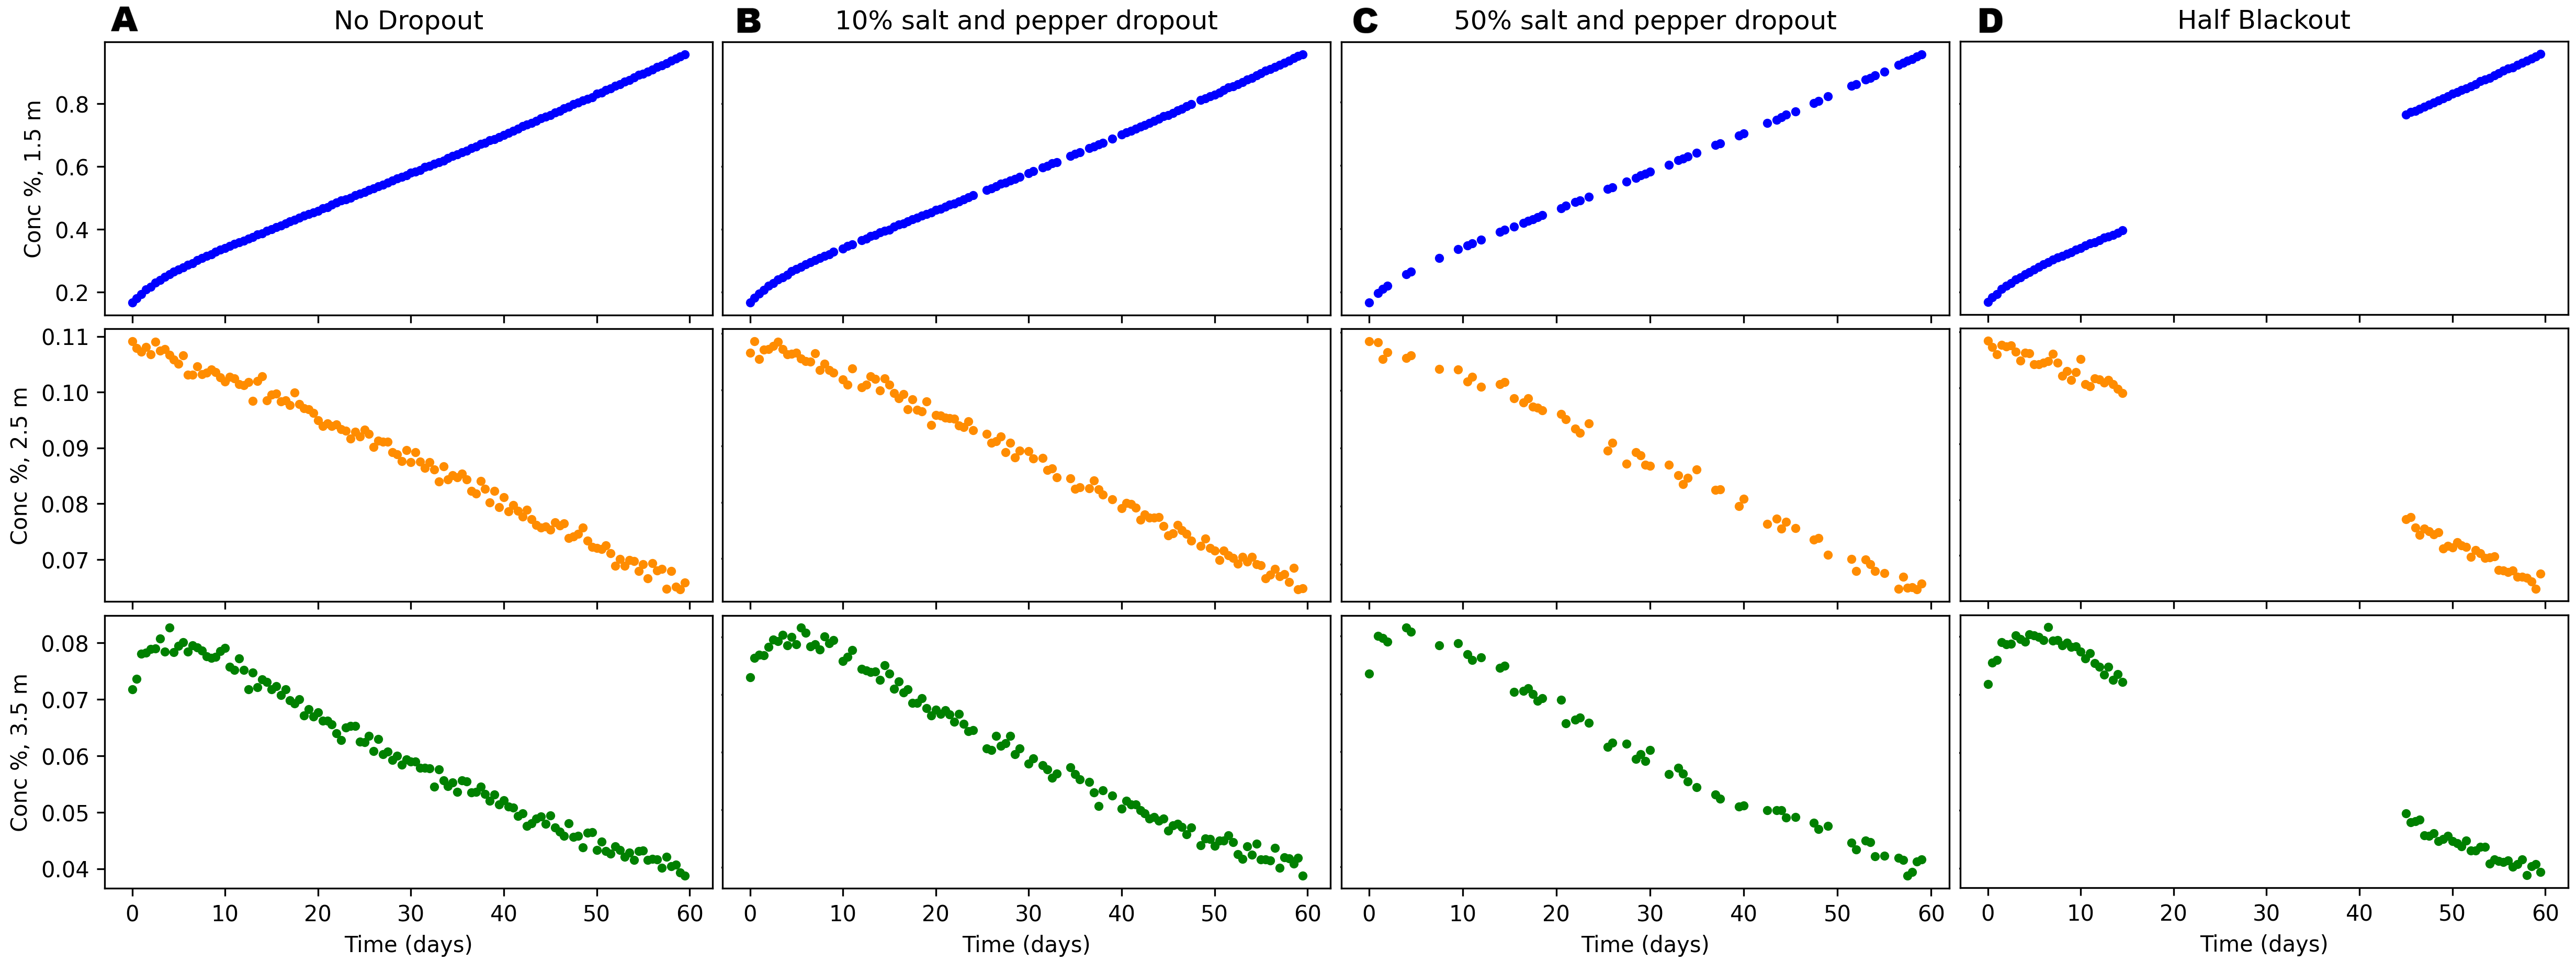
\includegraphics[width=6in]{figures/sens_dropout.png}
    \caption{Sensor dropout scenarios. (A) Base case with measurements every 12 hours. (B) Random removal of 10\% of measurements. (C) Random removal of 50\% of measurements (salt-and-pepper). (D) Contiguous removal of a block spanning 50\% of the recording period.}
    \label{fig:sim_sensDropout}
\end{figure}

\textcolor{red}{The comment here was not readable}

Evaluating the interpolation methods under sensor dropout is important because dropout is common in real-world deployments, ranging from single missing measurements to extended outages spanning days or weeks, as noted in Section~\ref{sec:real_data}. This manipulation is reasonable to test since it reflects deployment conditions already observed in the real-world dataset, rather than an artificial worst case. We evaluate whether the parameter estimation methods can still produce a realistic spatial distribution when fit against large, contiguous gaps in the temporal record, since their reliance on the full time series makes them more exposed to this kind of data loss. The distance-based interpolators are expected to be largely unaffected, as they do not substantially rely on temporal structure in the first place.


\section{Hyperparameter Tuning}
\label{sec:hyp_tuning}

Each of the five methods evaluated in this thesis depends on a small number of hyperparameters. These are configuration choices that are fixed before the method is executed and are not themselves learned from the data. Unlike the physical soil parameters estimated by the parameter estimation methods, hyperparameters govern how each method searches for a solution rather than describing the underlying soil system directly. Examples include the power parameter in IDW, the choice of variogram model in Kriging, and the number of iterations and pilot points used by the parameter estimation methods. Poorly chosen hyperparameters can degrade performance substantially, for example by causing a method to converge too slowly, overfit to the sparse temporal measurements, or fail to capture the correct spatial structure of the plume, so an appropriate set of values must be identified before the methods can be fairly compared.

Hyperparameter tuning is particularly important for the parameter estimation methods, 4D-Var, GLM, and IES, since these solve an iterative optimisation problem and are therefore sensitive to choices such as the number of pilot points and the number of iterations permitted before convergence. Too few pilot points limit the spatial resolution that can be recovered, while too many can lead to over-parameterisation given the sparse sensor network. Similarly, too few iterations may leave the optimisation under-converged, while too many can cause the method to overfit to the temporal measurements at the expense of spatial accuracy, as discussed further in Section~\ref{sec:fdvar_tuning}. The distance-based methods, IDW and Kriging, involve comparatively fewer and less consequential hyperparameters, though their tuning is still considered below for completeness.

To identify suitable values for each method, a grid search is performed over the relevant hyperparameters using a training subset of $\trainsize$ synthetic data samples, held separate from the samples used for final evaluation. For each combination of hyperparameters, the method is run across the training set and its spatial reconstruction error is recorded; the combination yielding the lowest error is then adopted for all subsequent evaluations of that method. The tuning procedure and results for each method are described in turn below.

 \subsection{Inverse Distance Weighting}
 \label{sec:idw_tuning}
 Given its role as a baseline method, hyperparameter tuning for IDW was kept minimal. A grid search over the power parameter $\idwpow \in \{1, 2, 4\}$ and the temporal averaging window $\idwwin \in \{1, 3, 5\}$ was performed on the training data. Results are shown in Figure~\ref{fig:idw_hyperp}.

   \begin{figure}[!h]
 \centering
 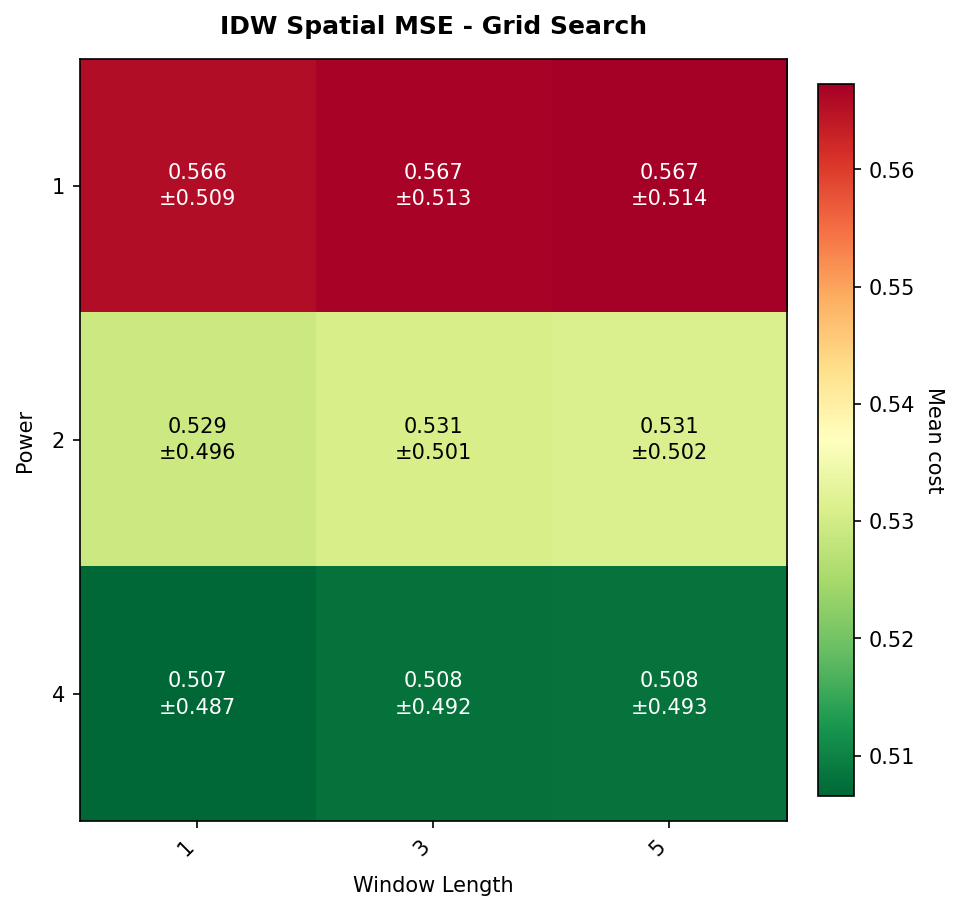
\includegraphics[width = 4in]{figures/idw_gridsearch.png}
 \caption{Hyperparameter search for inverse distance weighting parameters $\idwpow$ and $\idwwin$. The colorbar represents MSE of the spatial approximation vs the synthetic ground truth. Measurement noise=0.02 which is quite large to properly evaluate the averaging window.}
 \label{fig:idw_hyperp}
 \end{figure} 

 The results are straightforward. MSE decreases monotonically as the power increases. Powers beyond 4 were considered, but as shown in Figure~\ref{fig:idw_example}, a power of 4 already produces a discontinuous spatial distribution; higher values were therefore excluded to maintain physically realistic estimates. The grid search demonstrated that the window size has little effect on MSE, so a window of 3 is adopted to retain partial use of the temporal dimension.
 
\subsection{Kriging}
\label{sec:krig_tuning}
 
Hyperparameter tuning for Kriging was also limited, reflecting its role as a baseline and its modest performance in preliminary testing. The \trainsize-sample training set was used to identify the best combination of variogram fitting model and dissimilarity metric. The considered fitting models were linear, exponential, Gaussian, spherical, and an automatic selection scheme. These were evaluated against temporal semi-variance, single semi-variance, and Pearson correlation dissimilarity metrics as defined in Equations~\ref{eq:semVar2}, \ref{eq:semVar_more}, and \ref{eq:pearsonCorr}. The automatic selection computes the fitting error for each of the four parametric models and selects whichever achieves the lowest MSE against the empirical variogram.
 
\begin{figure}[!h]
    \centering
    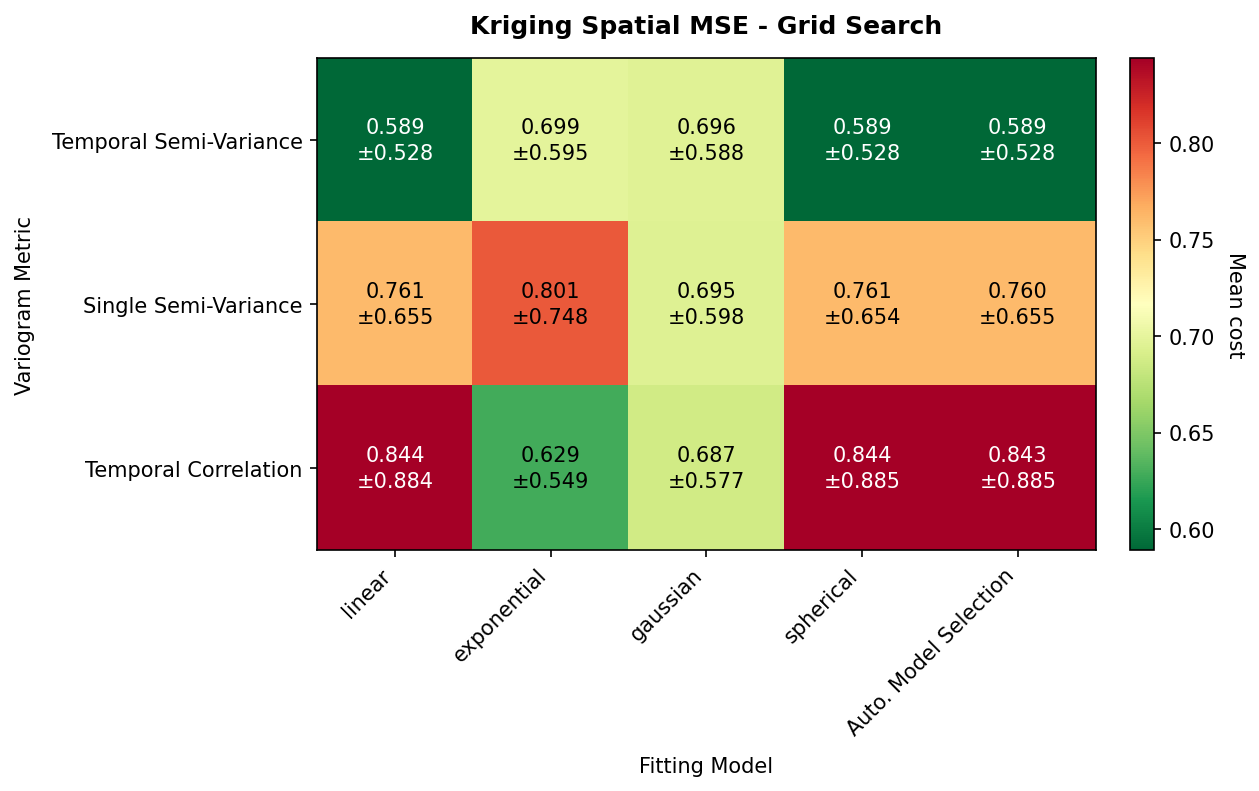
\includegraphics[width=5in]{figures/kriging_gridsearch.png}
    \caption{Grid search results for Kriging hyperparameters. The colourbar represents spatial MSE relative to the synthetic ground truth.}
    \label{fig:krig_hyperp}
\end{figure}
 
As shown in Figure~\ref{fig:krig_example}, the empirical variograms in this problem contain only 2--6 data points. With so few points, the spherical and linear models converge to the same line of best fit and produce identical scores. Likewise, the automatic selection consistently chooses one of these two and yields equivalent results. The Gaussian and exponential models proved unable to characterise these sparse empirical variograms accurately. Among the dissimilarity metrics, temporal semi-variance substantially outperformed the alternatives because it explicitly captures the temporal dimension of the data, which single semi-variance does not. Pearson correlation was also found to be inadequate. Based on these results, automatic model selection paired with temporal semi-variance (Equation~\ref{eq:semVar_more}) is adopted for all subsequent Kriging evaluations.
 
\subsection{4D-Var}
\label{sec:fdvar_tuning}
 
Unlike the distance-based methods above, 4D-Var exploits the full temporal structure of the data. A visual illustration of this process is provided in Figure~\ref{fig:fdvar_temporal_example}. Hyperparameter tuning of 4D-Var considered the maximum number of iterations $\numIterations$ and the number of pilot points $\npp$, with a grid search over $\numIterations \in \{100, 250, 500, 1000\}$ and $\npp \in \{3, 5, 8, 10\}$.
 
\begin{figure}[!h]
    \centering
    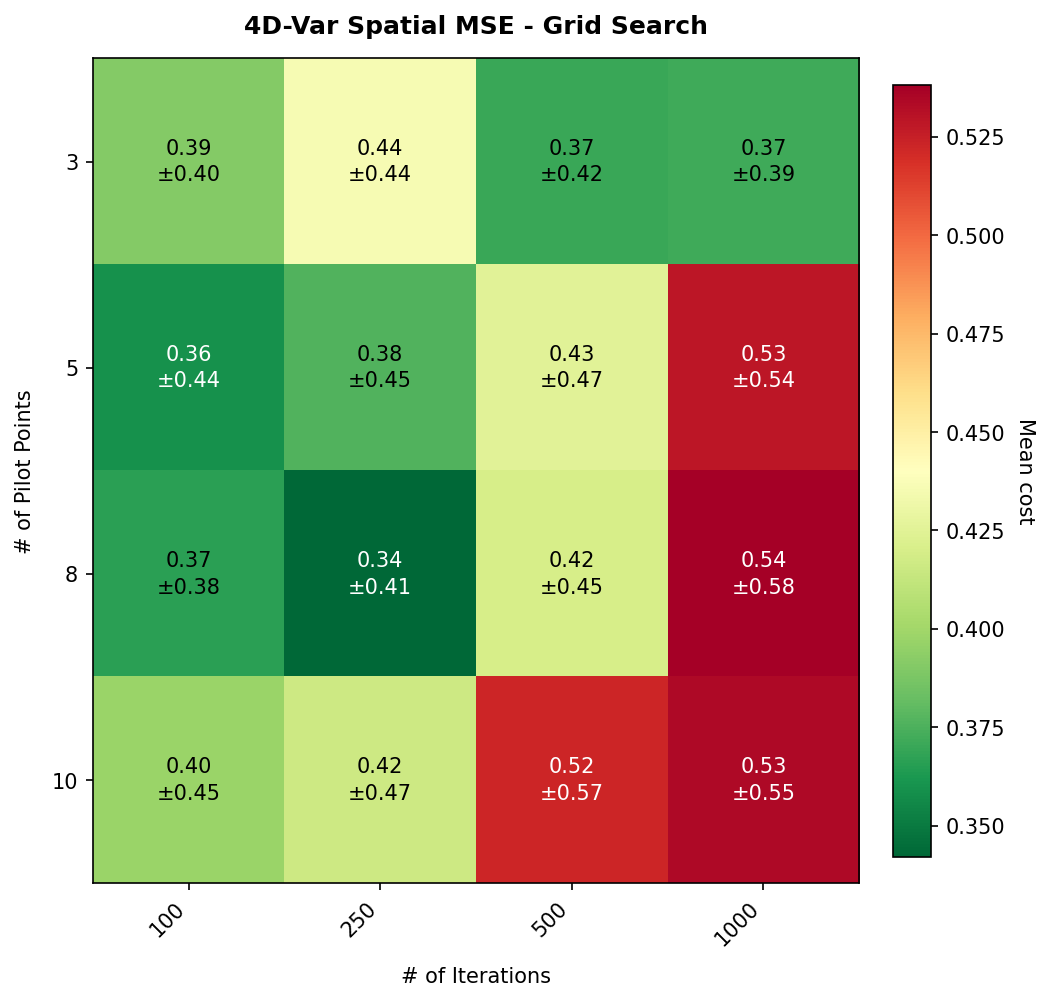
\includegraphics[width=5in]{figures/fdvar_spat_gridsearch_means.png}
    \caption{Hyperparameter grid search for 4D-Var. Spatial error between $\conc$ and $\hat{\conc}_\nSampTime$ after temporal calibration.}
    \label{fig:fdvar_spat_gridsearch}
\end{figure}
 
The corresponding temporal error plot is provided in Appendix Figure~\ref{fig:fdvar_temp_gridsearch}, and shows the expected result. Both more iterations and more pilot points reduce temporal fitting error; however, Figure~\ref{fig:fdvar_spat_gridsearch} reveals a different trend when evaluated spatially. Beyond 250 iterations, the parameter estimation process over-fits to the temporal data, producing solutions that are too constrained, driving spatial error upward. The best-performing combination is 8 pilot points and 250 iterations, though neighbouring configurations perform comparably. These values are used for all subsequent 4D-Var evaluations.
 
Several additional hyperparameters such as learning rate, the optimisation algorithm, and parameter priors were held fixed rather than searched to limit complexity. A learning rate of 0.01 was selected for its widespread use and moderately aggressive momentum~\cite{learningRates}. The ADAM optimiser was used to compute parameter updates~\cite{AdamPaper} given the gradient. Priors for initial PHC concentrations are set from the first available measurements at each sensor location, with values at unsensed depths obtained by interpolation. Source boundary concentrations are initialised at 0.1\% to discourage the method from biasing towards high boundary condition values. The soil parameters $\advecCoeff$, $\biodegCoeff$, and $\diffCoeff$ are initialised at the midpoint of their respective ranges, giving values of $0$, $0$, and $10^{-8}$---a standard choice in the absence of prior information~\cite{pestManual}. More informative priors could be derived from auxiliary data, but this is beyond the scope of the present work.
 
 
\subsection{GLM}
\label{sec:glm_tuning}
 
The GLM algorithm closely parallels 4D-Var. It is a forward simulation is fitted to the temporal observations by minimising the cost function in Equation~\ref{eq:paramEst_costFunc}. The key difference lies in how parameter sensitivities are estimated. As described in Section~\ref{sec:background_glm}, GLM approximates gradients by perturbing each parameter by a small amount and recording the resulting change in cost, rather than computing gradients analytically.
 
Hyperparameter tuning followed the same process as 4D-Var, searching over $\npp \in \{3, 5, 8, 10\}$ pilot points and $\numIterations \in \{10, 20, 30, 40\}$ iterations.
 
\begin{figure}[!h]
    \centering
    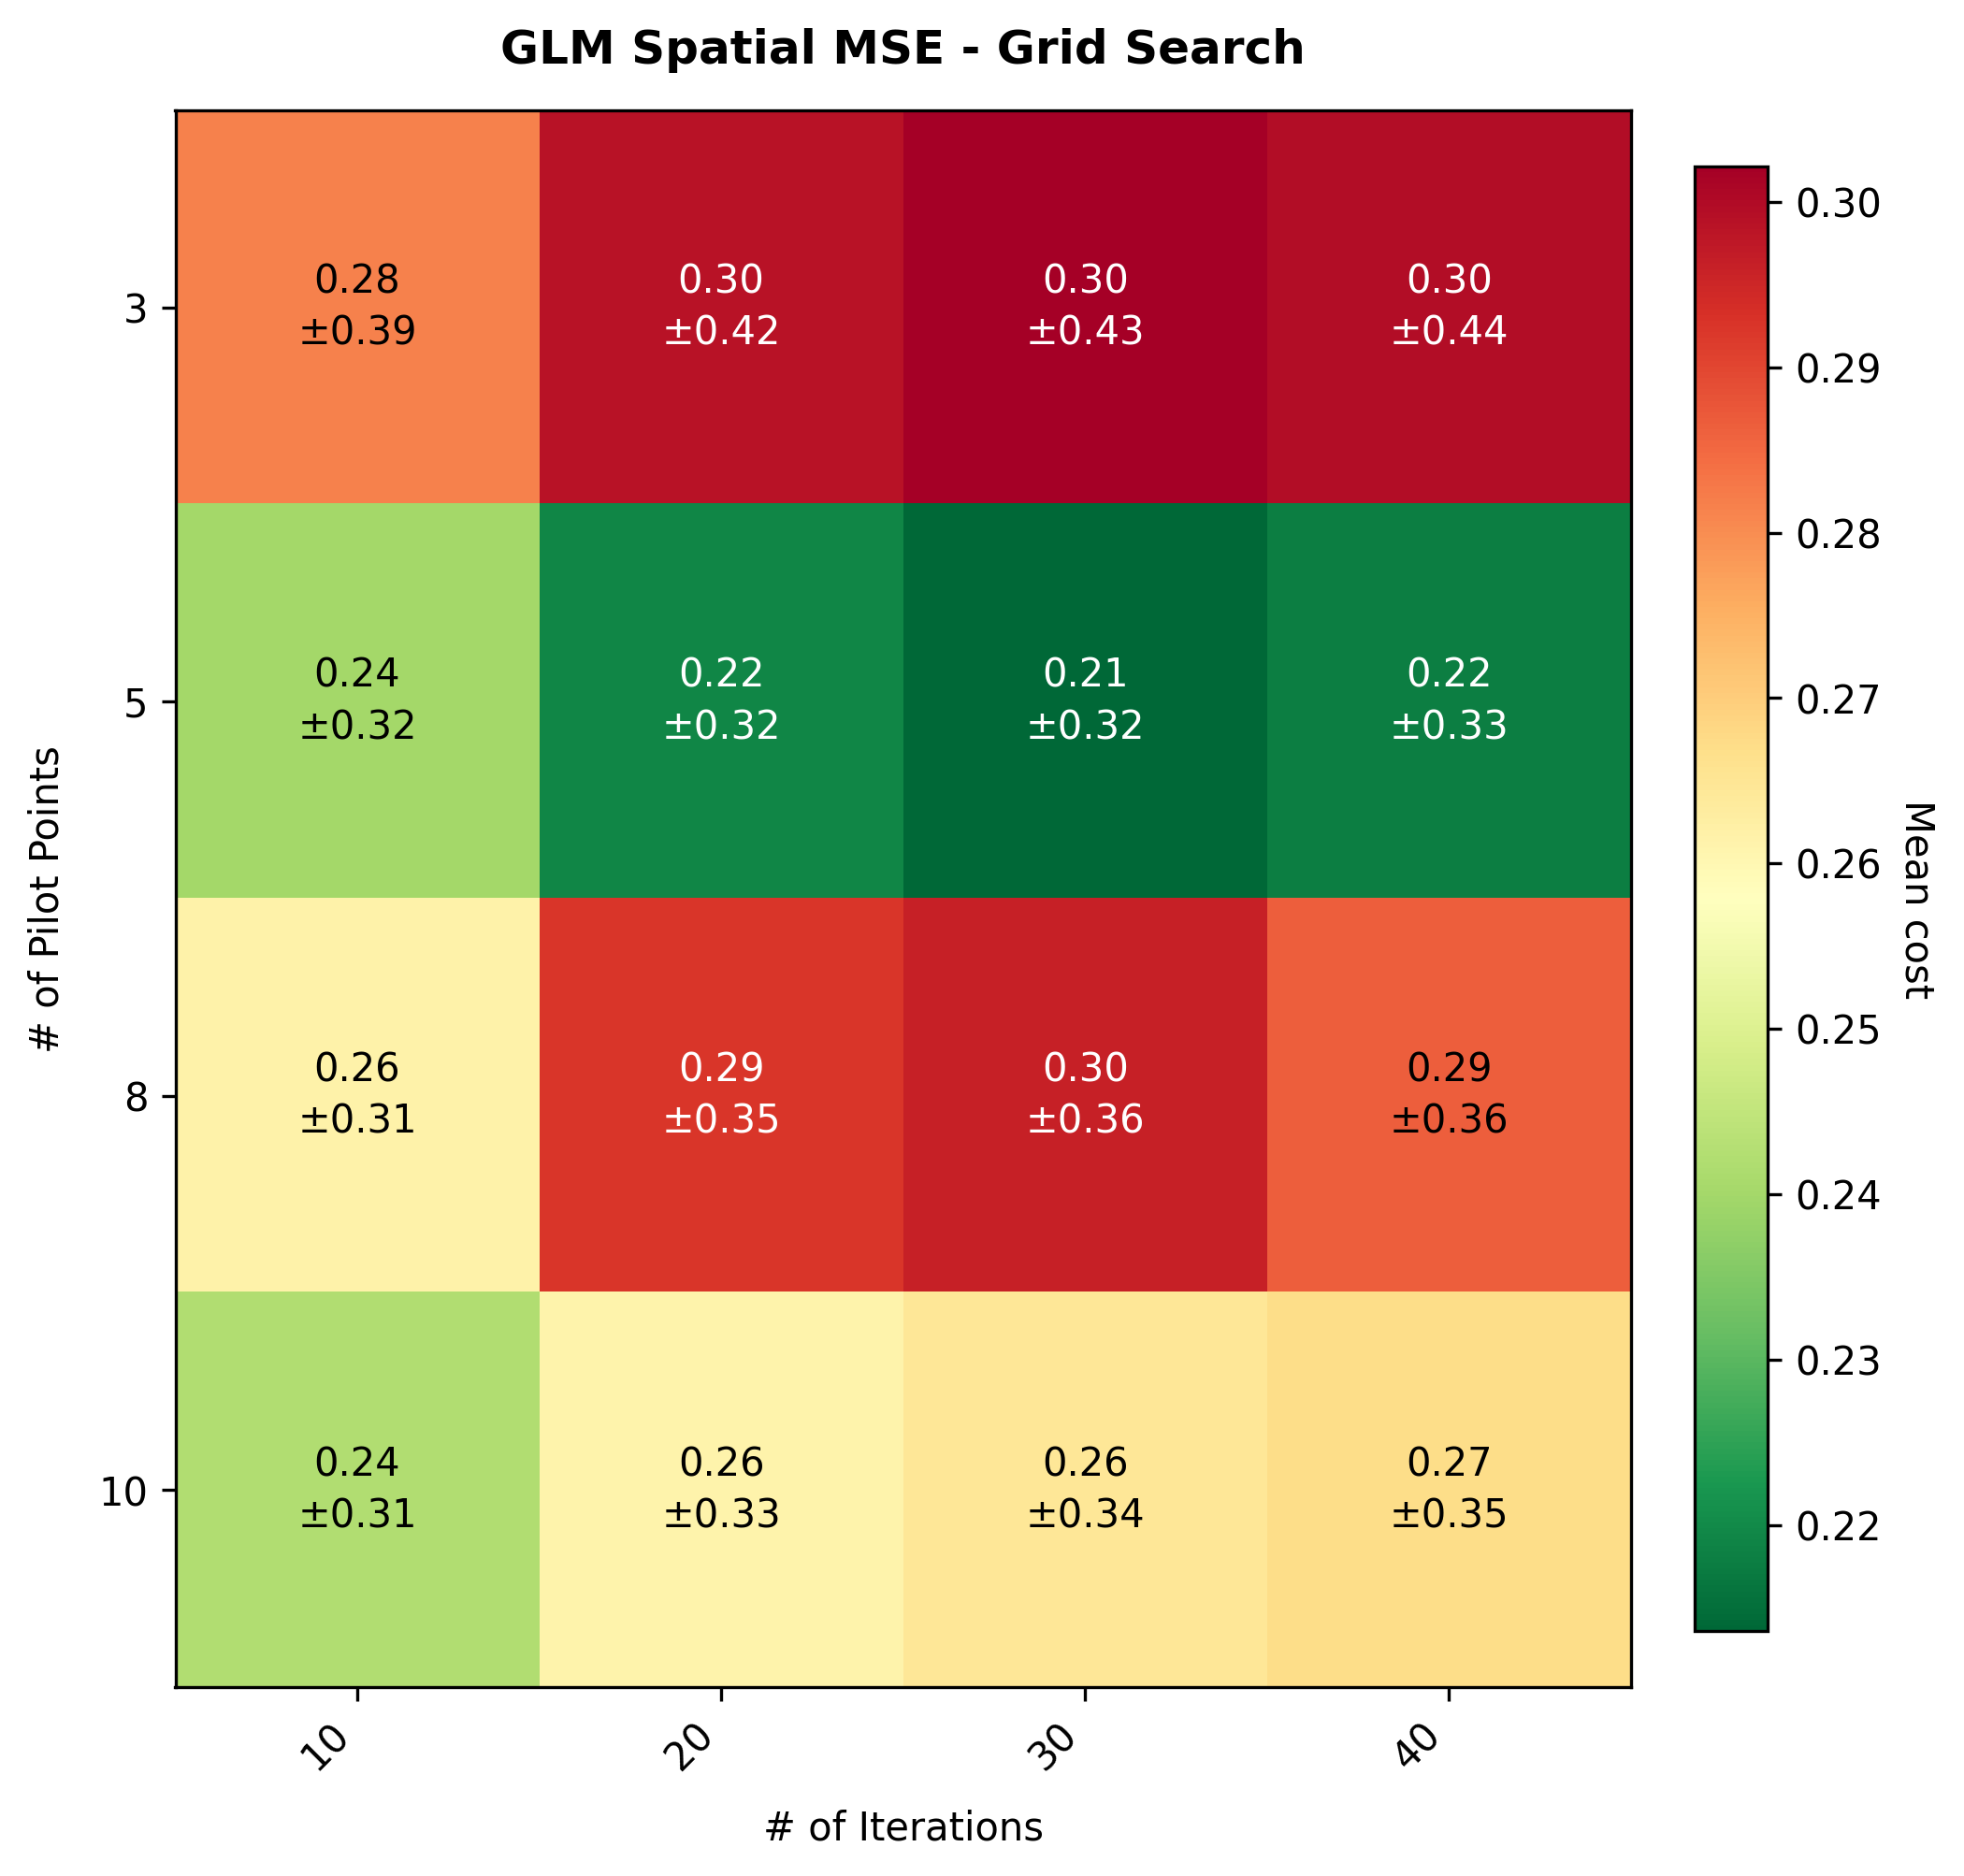
\includegraphics[width=5in]{figures/glm_spat_gridsearch.png}
    \caption{Hyperparameter grid search for GLM. Spatial error between $\conc$ and $\hat{\conc}_\nSampTime$ after temporal calibration.}
    \label{fig:glm_spat_gridsearch}
\end{figure}
 
The results are more decisive than those of 4D-Var. Five pilot produces spatial errors at least 33\% lower than all other values. The iteration count shows less differentiation where 30 iterations yields the lowest MSE, but results at 10 and 20 are close, within 5\%; well within the standard error of the test. To reduce computation time, 5 pilot points and 20 iterations are adopted for all subsequent GLM evaluations.
 
 
\subsection{Iterative Ensemble Smoother}
\label{sec:ies_tuning}
 
IES is the last of the parameter estimation methods. It maintains an ensemble of parameter vectors, uses their covariance structure to guide updates, and iterates toward the minimum temporal error. Given the consistent finding of 5 optimal pilot points in the preceding sections, this hyperparameter is not re-searched here. Instead, the grid search focuses on the number of iterations and ensemble size, testing $\numIterations \in \{5, 10, 15, 20\}$ and ensemble sizes of $\{50, 100, 150, 200\}$.
 
\begin{figure}[!h]
    \centering
    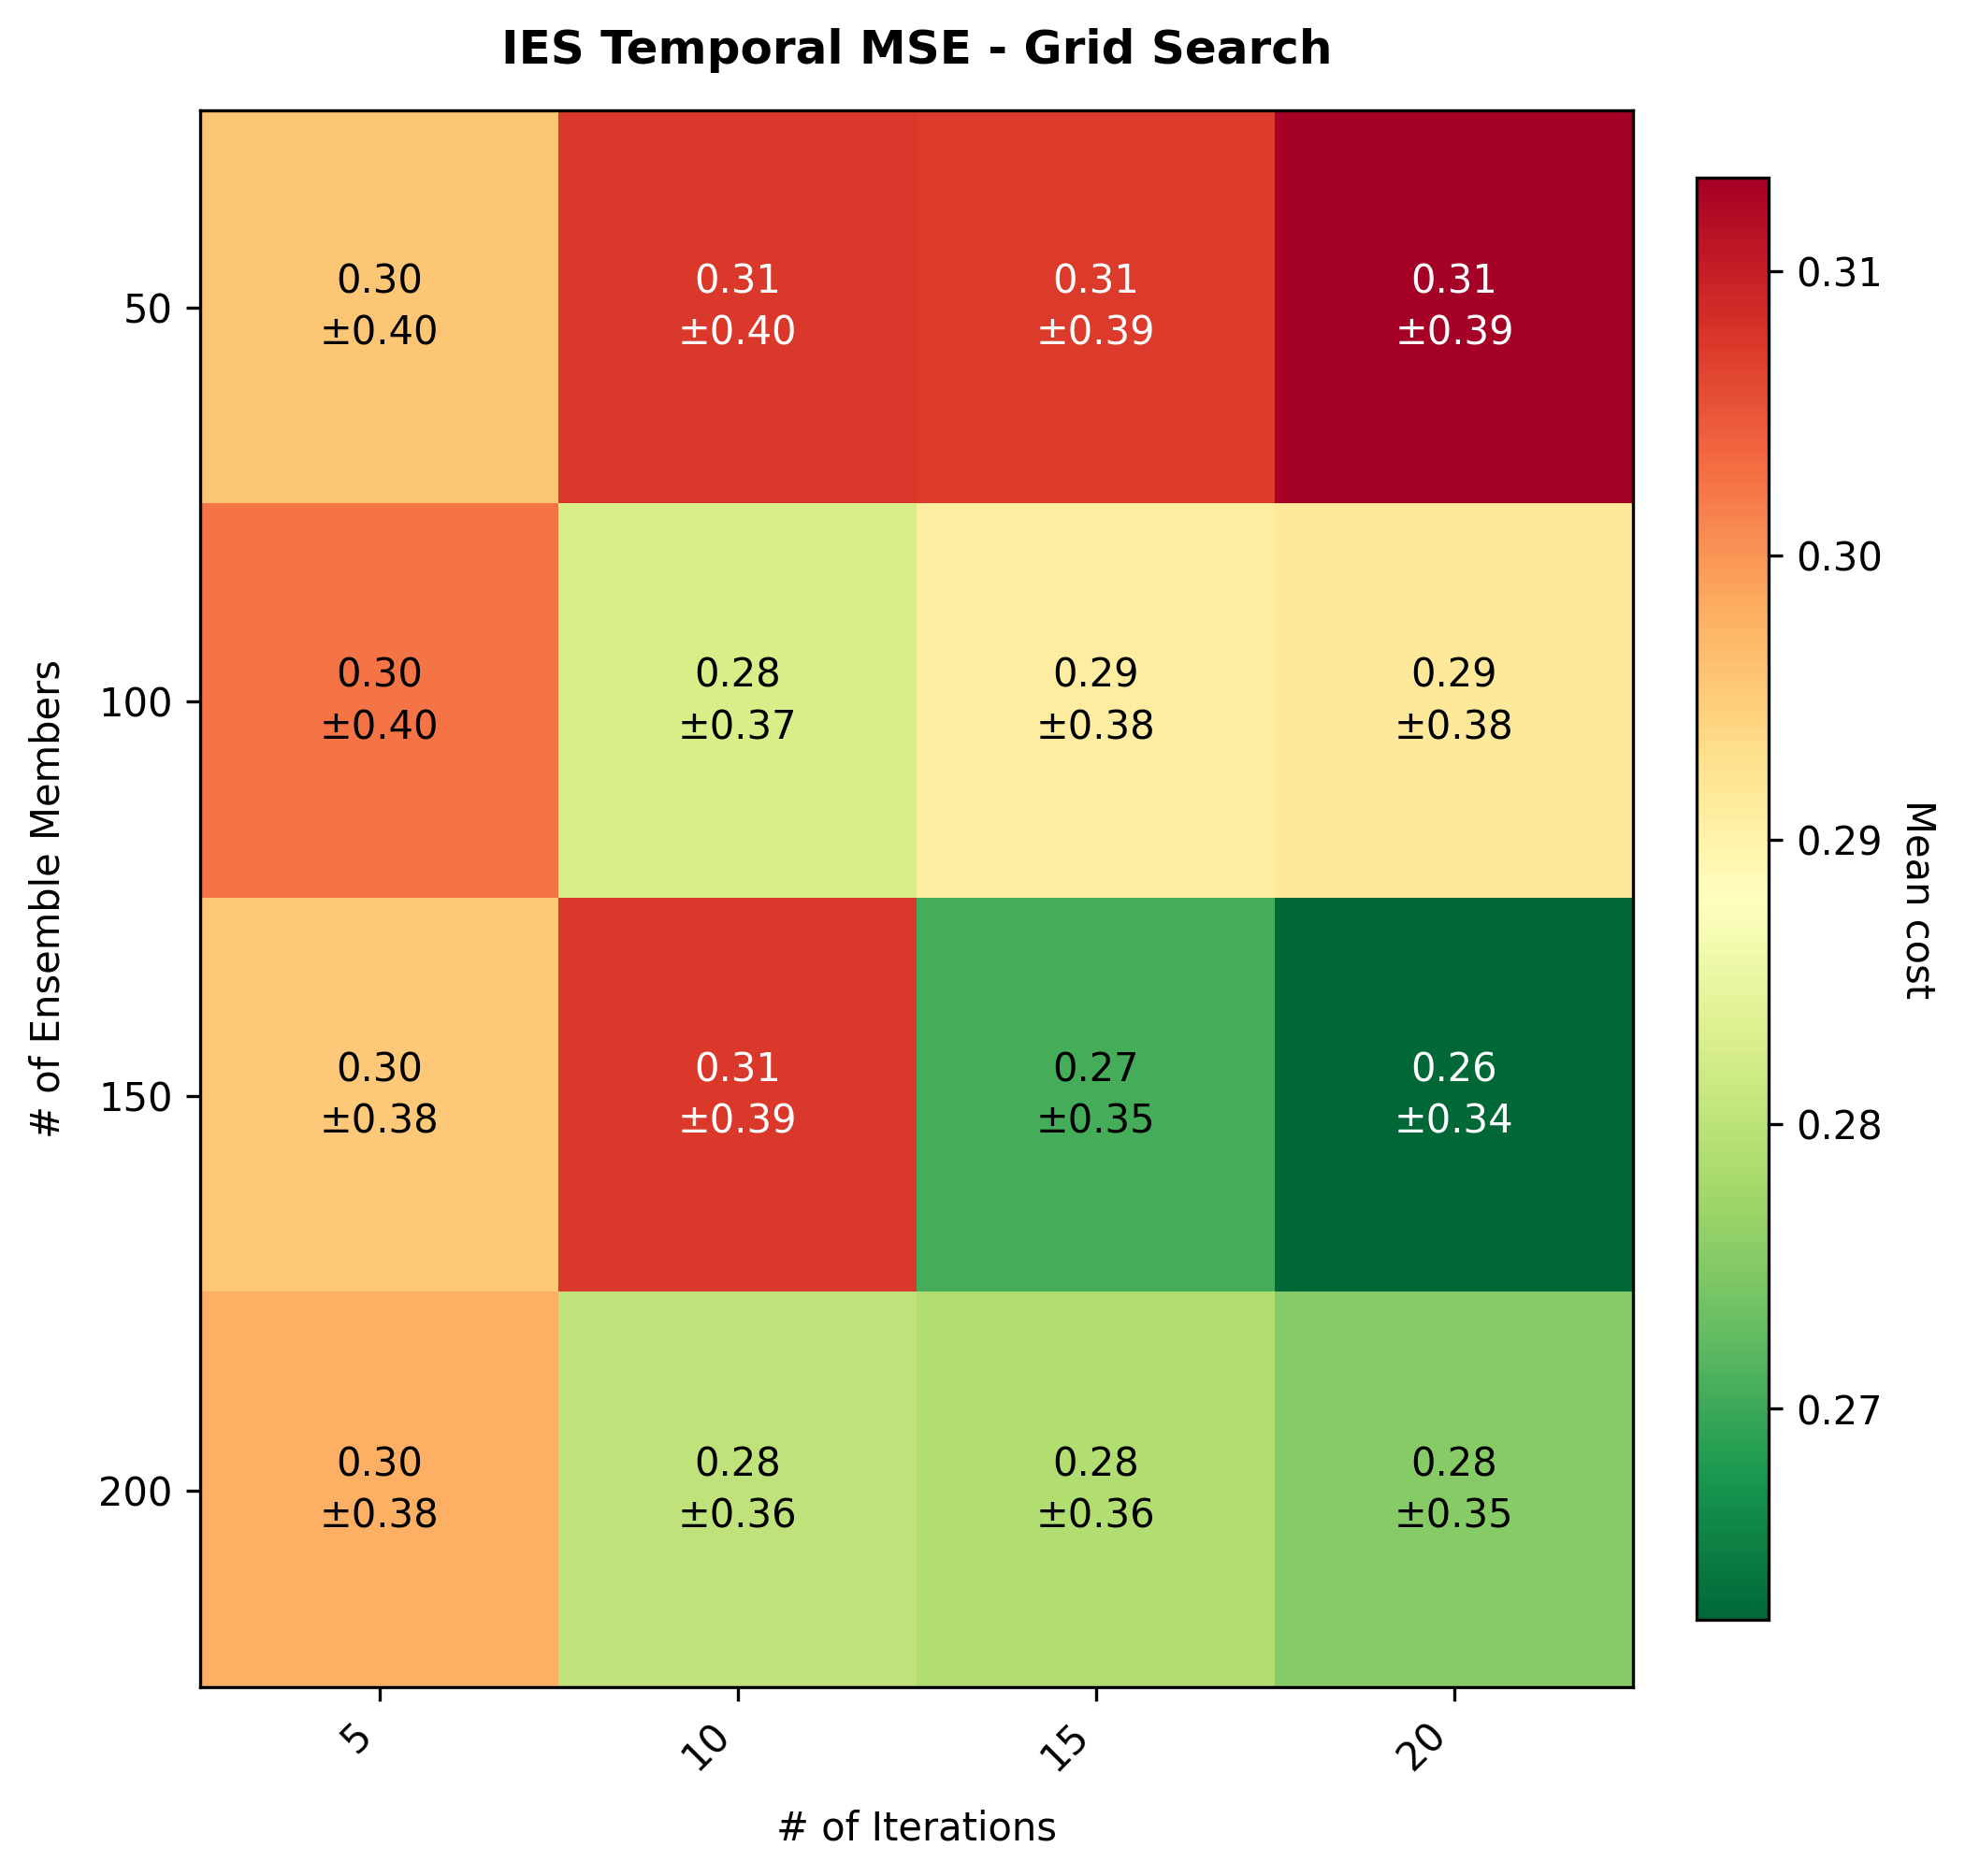
\includegraphics[width=5in]{figures/ies_spat_gridsearch.png}
    \caption{Hyperparameter grid search for IES. Spatial error between $\conc$ and $\hat{\conc}_\nSampTime$ after temporal calibration.}
    \label{fig:ies_spat_gridsearch}
\end{figure}
 
Spatial error generally decreases as both ensemble size and iteration count increase, but neither trend is as pronounced as in 4D-Var or GLM. Notably, spatial error appears to plateau quickly with increasing iterations, suggesting that ensemble size should be prioritised when computational budget is limited. As IES is the most expensive method evaluated, 200 ensemble members at 10 iterations are used in all subsequent tests as a practical balance between cost and performance.